\section{Evaluation}
To validate our analysis, we performed an extensive experimental evaluation of the algorithms described in the 
previous sections. We have implemented those algorithms in Hadoop 1.0.3 based on the description provided in their 
respective papers. \TODO{Hardware?}\\
All experiments were ran using two different datasets. The first one  
involves geographic XML data in two dimensions\footnote{Taken from \url{www.download.geofabrik.de}}. The second one is composed of image feature descriptors that we generated 
with the SURF \cite{SURF} technique\footnote{Images are taken 
from  \url{www.vision.caltech.edu/Image_Datasets/Caltech101}}, leading to data in dimension 128. 
Several parameters can impact the performance of computing kNN on MapReduce. We will focus on the size of the 
input data in number of records for both $R$ and $S$, the number of machines used in the MapReduce cluster (thereafter 
number of \emph{nodes}), the value of $k$ of the kNN query. Unless specified otherwise, we have used 20 nodes with $k=20$ 
in the following experiments. 

\subsection{Geographic dataset}
\subsubsection{Impact of input data size}
Our first set of experiments measure the impact of the data size on execution time, disk space and accuracy. 
 %Fichier généré par excel/NB_DATA.xls
 %Avec données datares/geo/all-2/
 %Fichier python perf/src/geo/timebydata.py
\paragraph*{Execution time} 
 %\begin{itemize}
%\item  \textbf{Impact on the time}
\begin{figure}[!h]
   \centering
    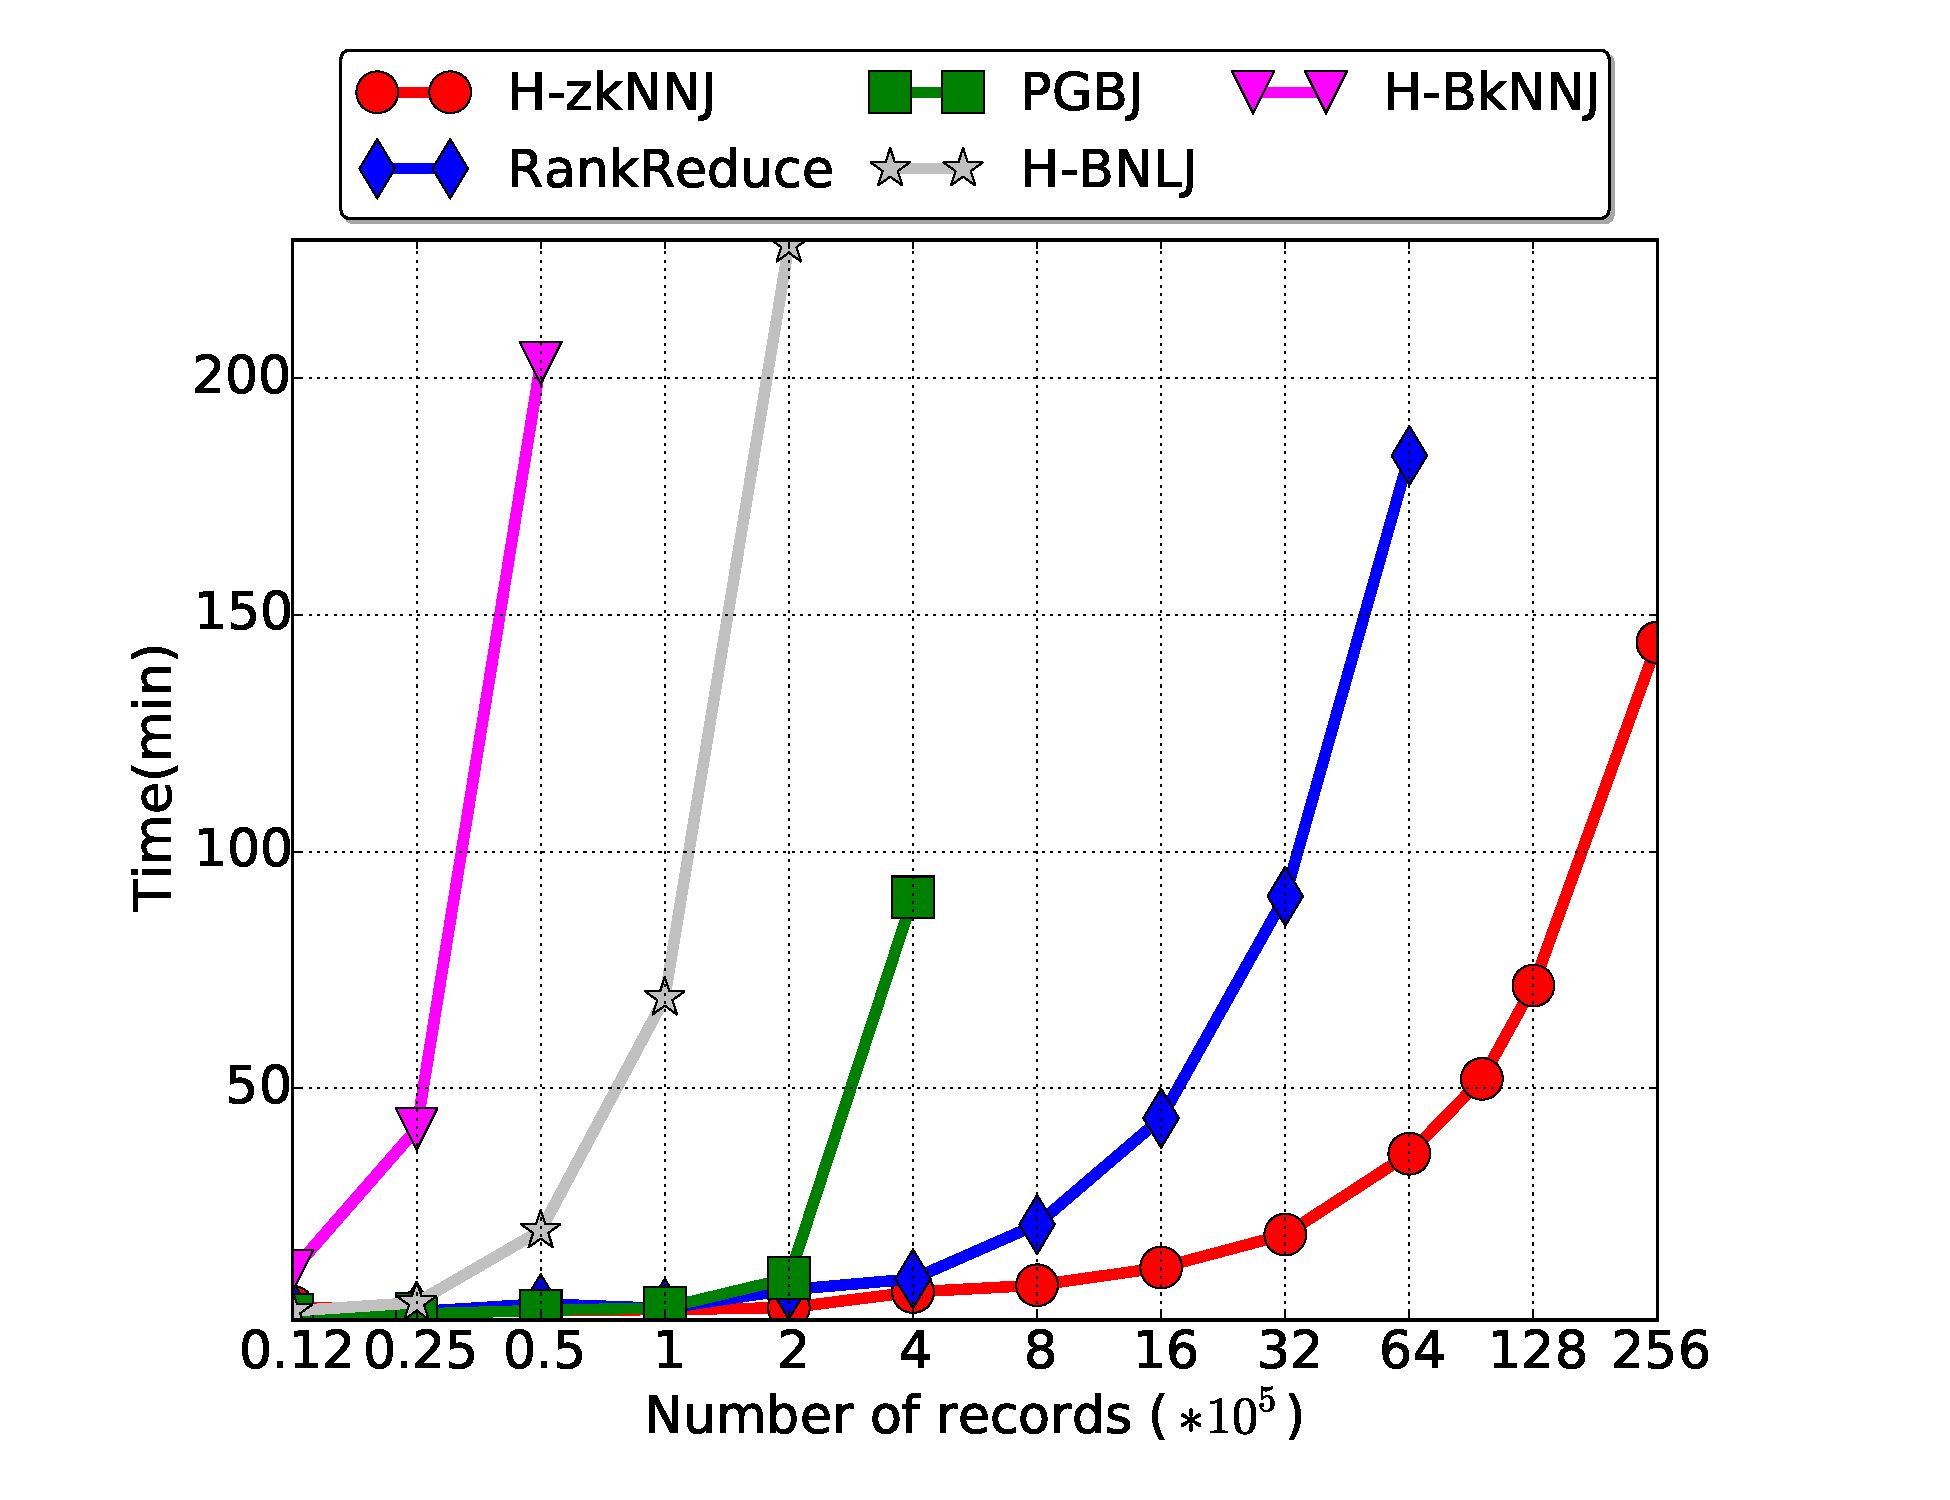
\includegraphics[scale=0.28]{img-perf/geo/data/time.pdf} 
     \caption{Geo data - Execution time\label{geo_data_time}}
\end{figure}

%The number of data deals in the same manner for all the algorithms.The time increases exponentially. For this performance, the algorithms are ranked by this order, H-BKNNJ ,H-BNLJ, Pgbj, H-LSH,H-ZKNNJ. But for the small dataset, it's more interesting to use PGBJ that has the same time that the  approximates methods.\\ For a dataset with $(>2*10^{5})$.Then,L-SH is better but increases more quickly that H-ZKNNJ and thus,at the end, this last method is better.\\
Figure~\ref{geo_data_time} shows the global computing time of all algorithms, varying the 
the number of records from $0.1*10^{5}$ to $256*10^{5}$. The global computing time increases more or less exponentially for 
all algorithms, but only H-zkNNJ and RankReduce can process medium to large dataset. For small dataset, PGBJ can compute an 
exact solution as fast as the other algorithms. 
\paragraph*{Disk Space}
%\item \textbf{Impact of the algorithms on the memory} 
        
\begin{figure}[!h]
 \centering
  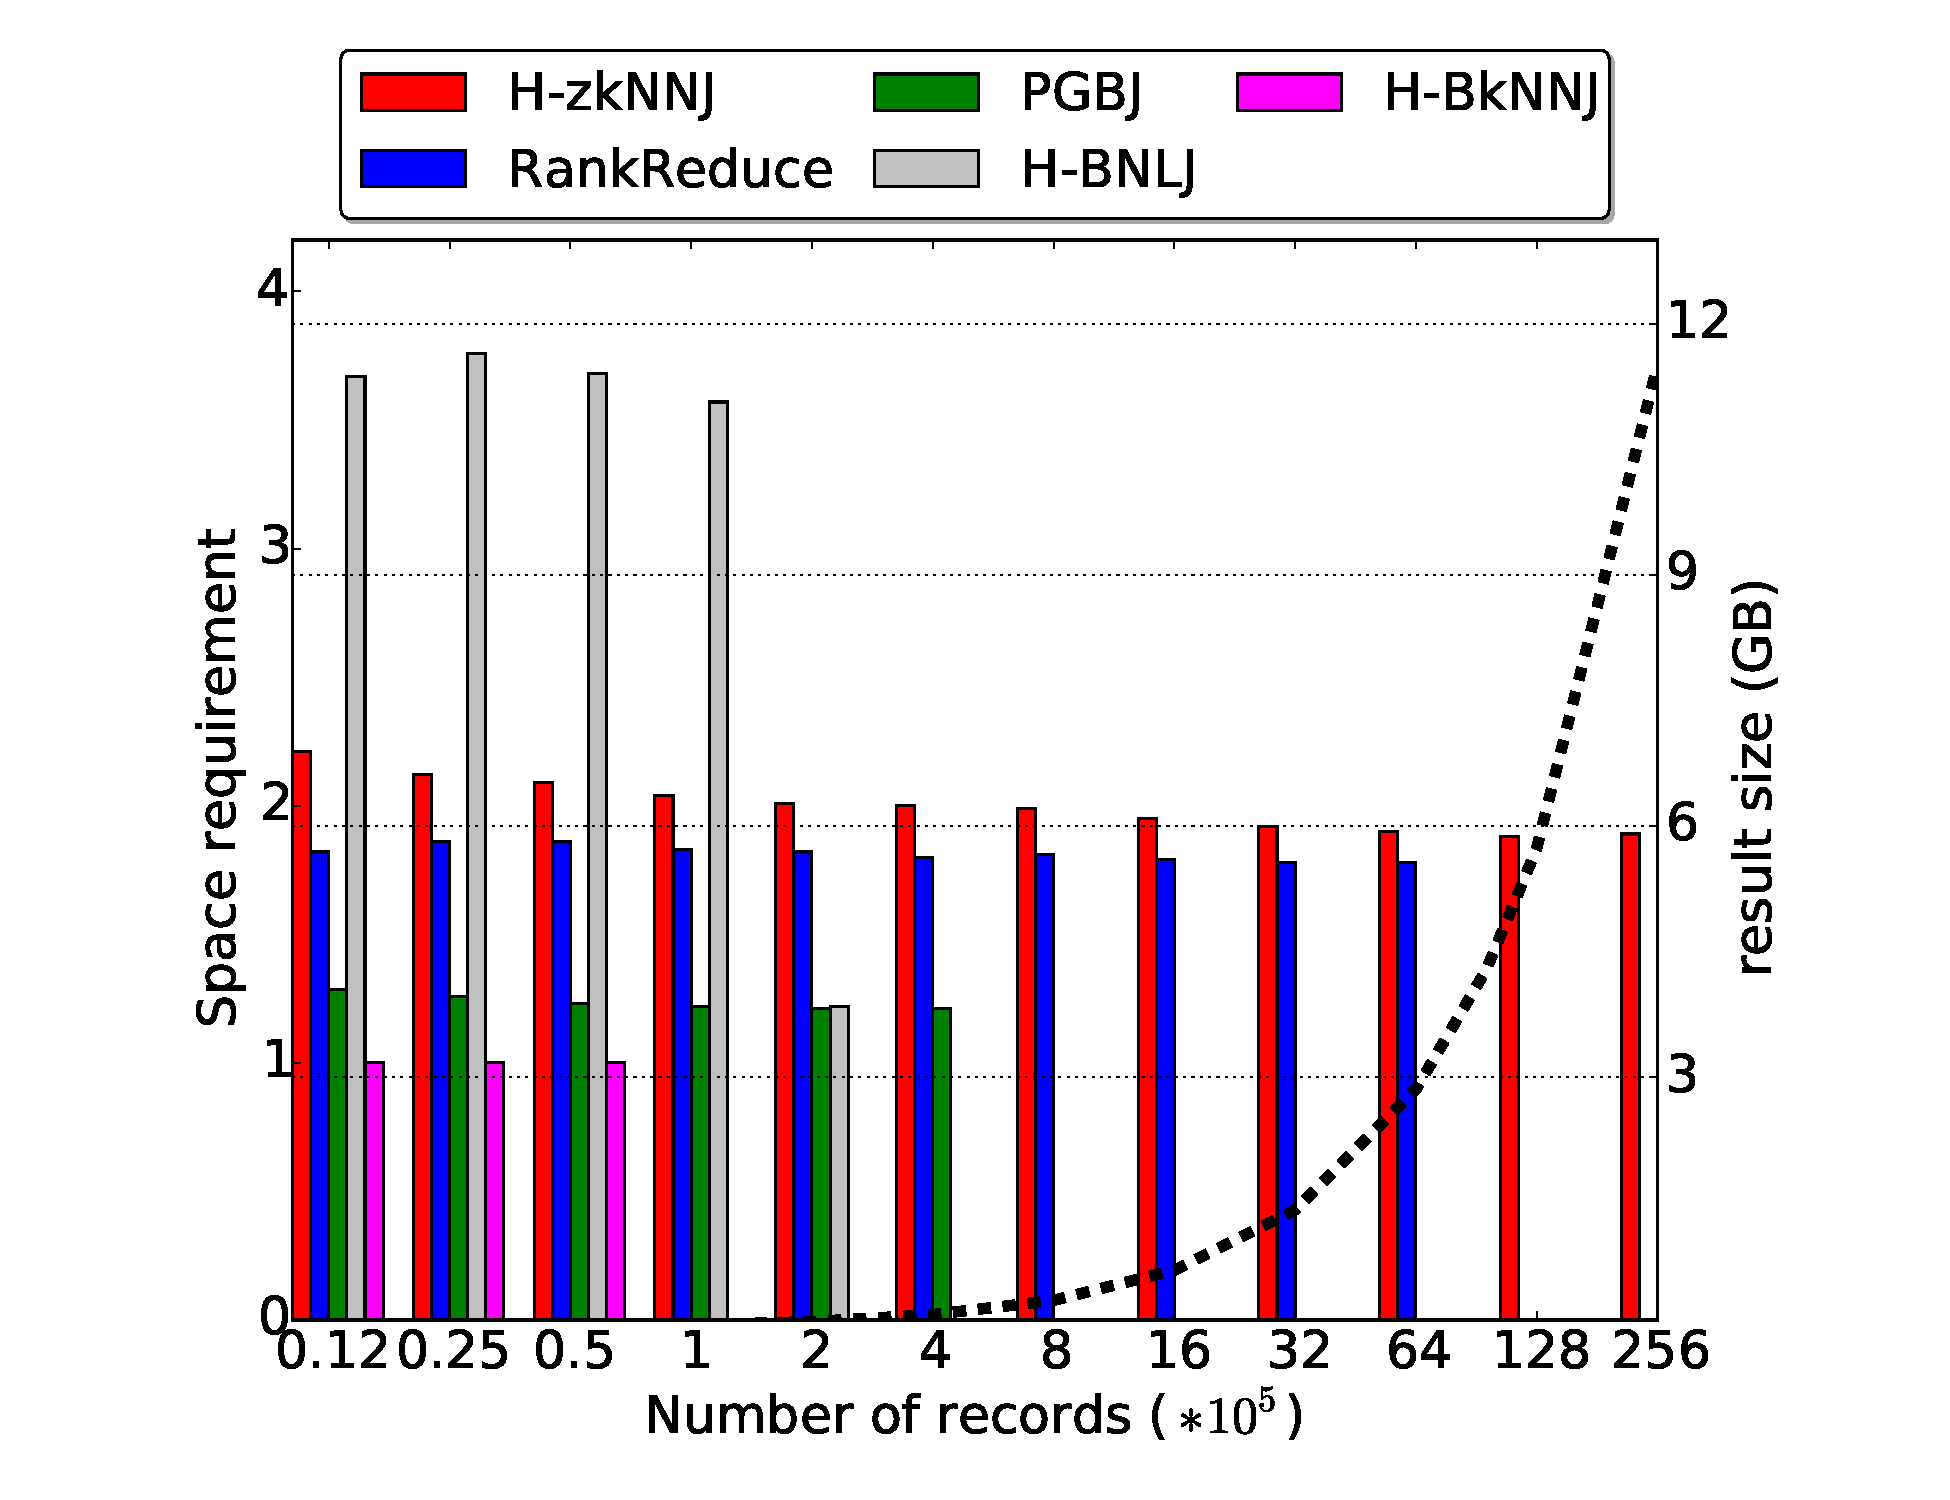
\includegraphics[scale=0.30]{img-perf/geo/data/memory.pdf} 
  \caption{Geo data - Space\label{geo_data_disk}}
\end{figure}%
      
Figure~\ref{geo_data_disk} shows the space requirements of each algorithms as a function of the final output size. To 
reduce the footprint of each run, intermediate data are compressed. We 
measure the intermediate data size and compute the ratio $\frac{T_{intermediate}+T_{final}}{T_{final}}$. For example, for 
H-BNLJ, the size of intermediate data is $1.6$ times bigger than the size of output data. Overall, the algorithms with the
lowest space requirements are RankReduce and PGBJ.
% because more data end in the same bucket, reducing data replication. On
%the other hand, H-BNLJ has an almost constant replication factor, depending on the number of partition chosen. 

%We can draw several conclusions from this figure:
%H-BNLJ consumes a lot of memory because of its constant replication of data (equals to number to partition chosen). As for 
%H-zkNNJ, its data replication pattern is not constant, therefore the ratio for h-zkNNJ decreases with the number of data. 
%The reason for this decrease is that more data are in a same bucket so less replication is needed.
%The same observation can be made for PGBJ. Nevertheless, it requires less memory thanks to its data replication 
%technique.\\ H-LSH uses a constant data replication pattern, thus the ratio of its required memory is constant.\\
        
     
       \begin{figure}[!h]
         \centering
         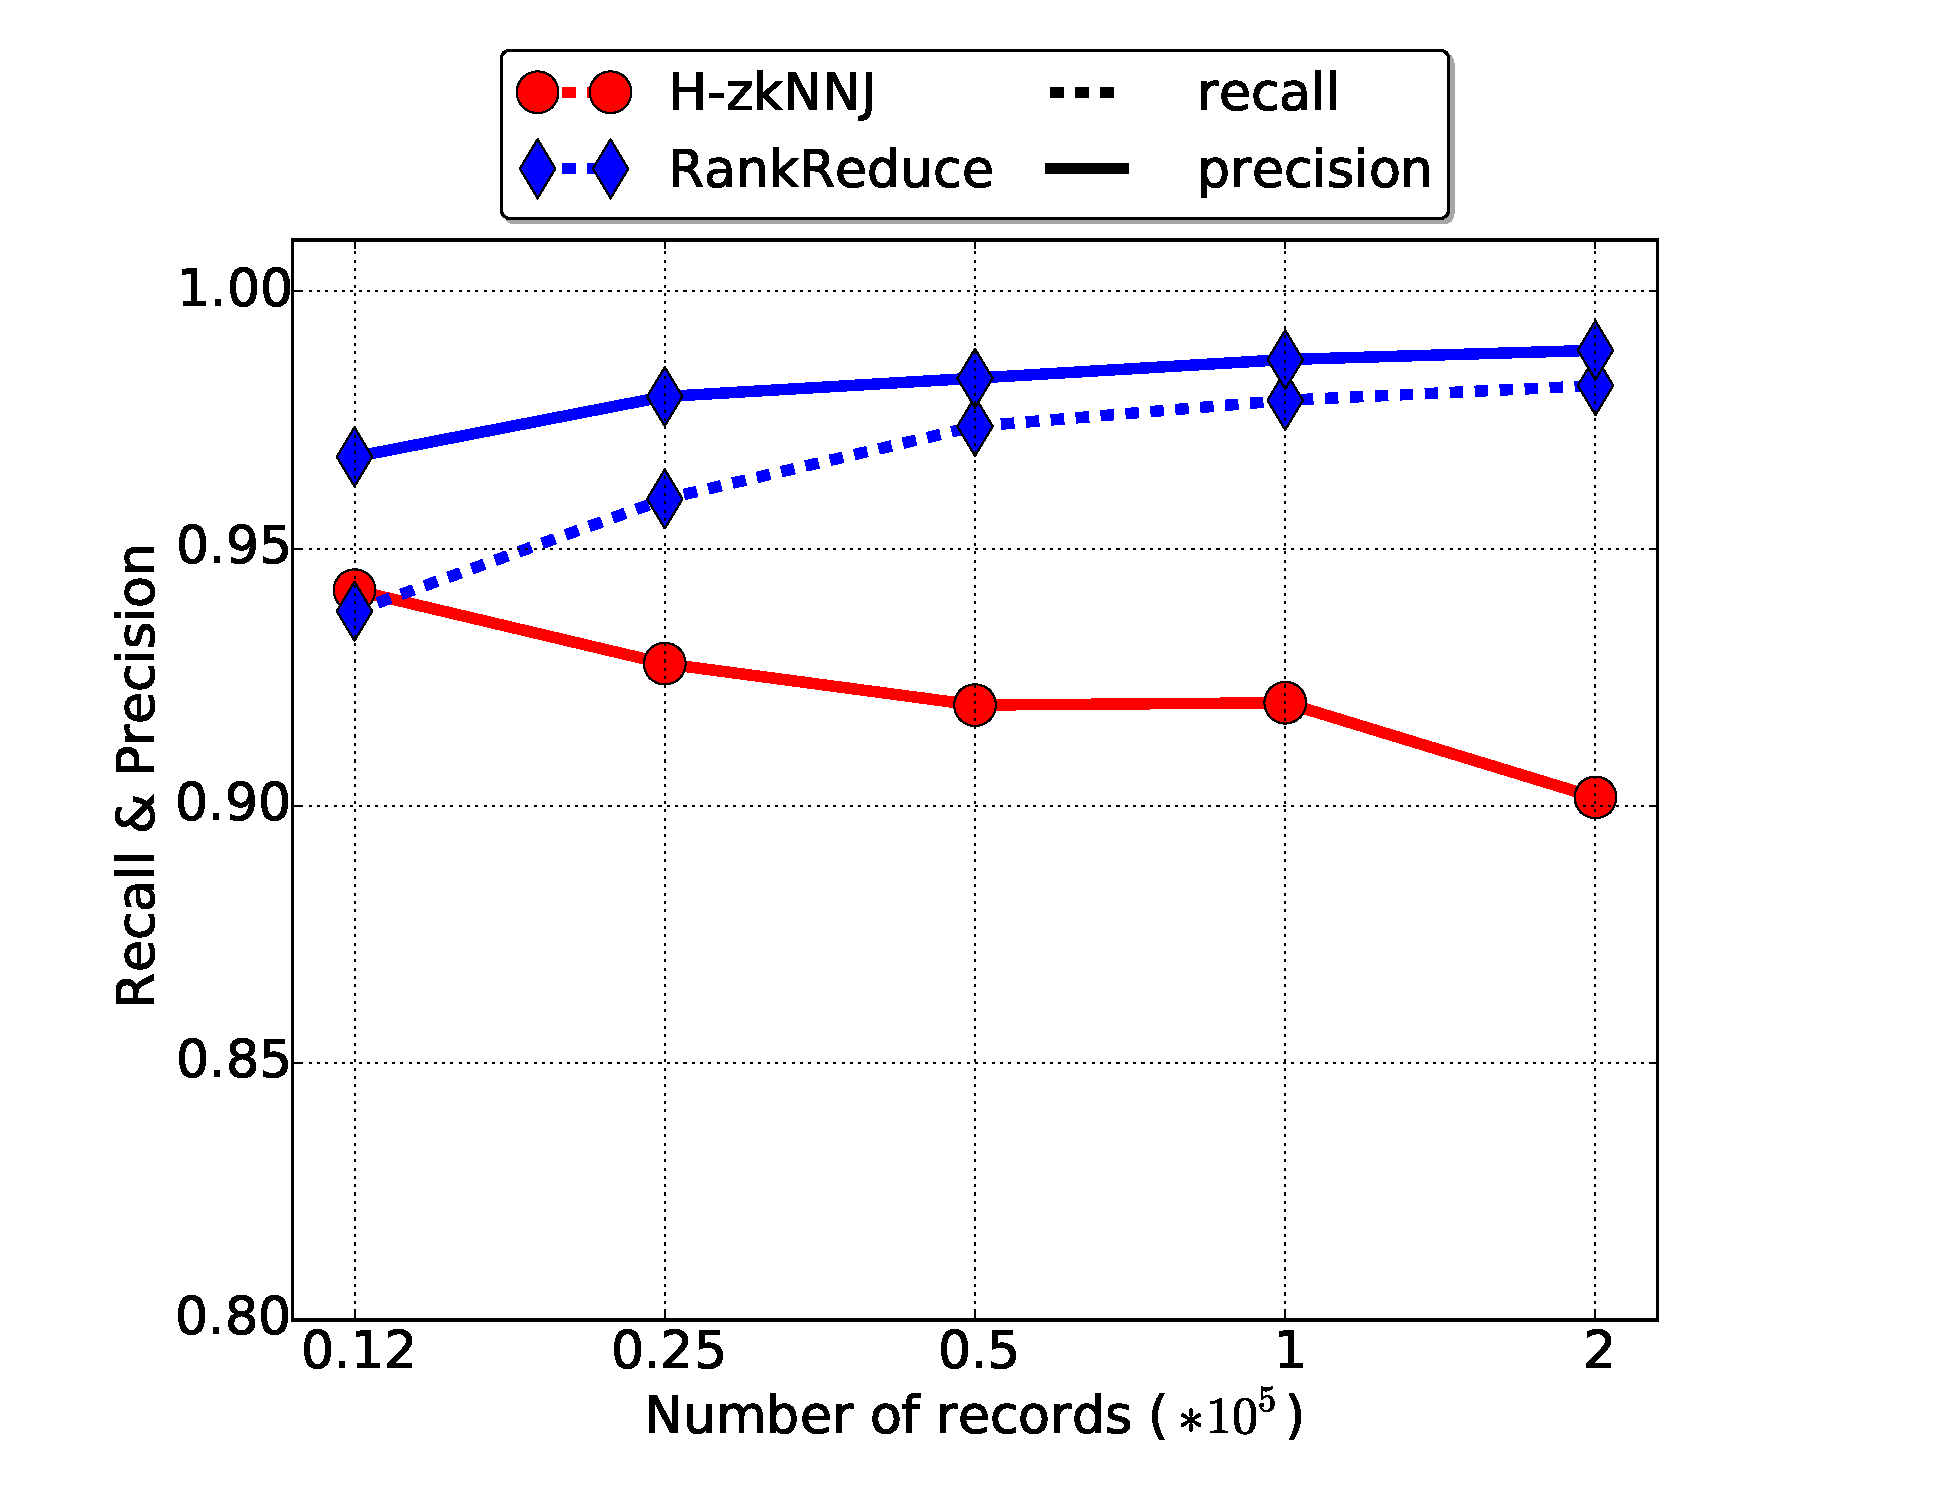
\includegraphics[width=0.52\textwidth]{img-perf/geo/data/accuracy.pdf} 
         \caption{Geo data - Accuracy\label{geo_data_accuracy}}
        \end{figure}
     
\paragraph*{Accuracy}     
     %      \item \textbf{ Impact on the accuracy :}
Figure~\ref{geo_data_accuracy} shows the accuracy of the two approximate algorithms, H-zkNNJ and RankReduce.
As the number of records increases, the accuracy of H-zkNNJ starts to decrease, while still being high (\TODO{why?}). 
On the other hand, RankReduce benefits from larger datasets because more data end up in the same bucket, increasing the number or candidates. 

\subsubsection{Number of computing nodes}
We now evaluate the optimal number of nodes to use in the computation by measuring the overall computing time using three 
different input data sizes for all algorithms.
\begin{figure}[!h]
 \centering
 %Fichier généré par excel/Nodes.xlsx 
 %Avec données datares/geo/nodes/
 %Fichier python perf/src/geo/timebyNodes.py
 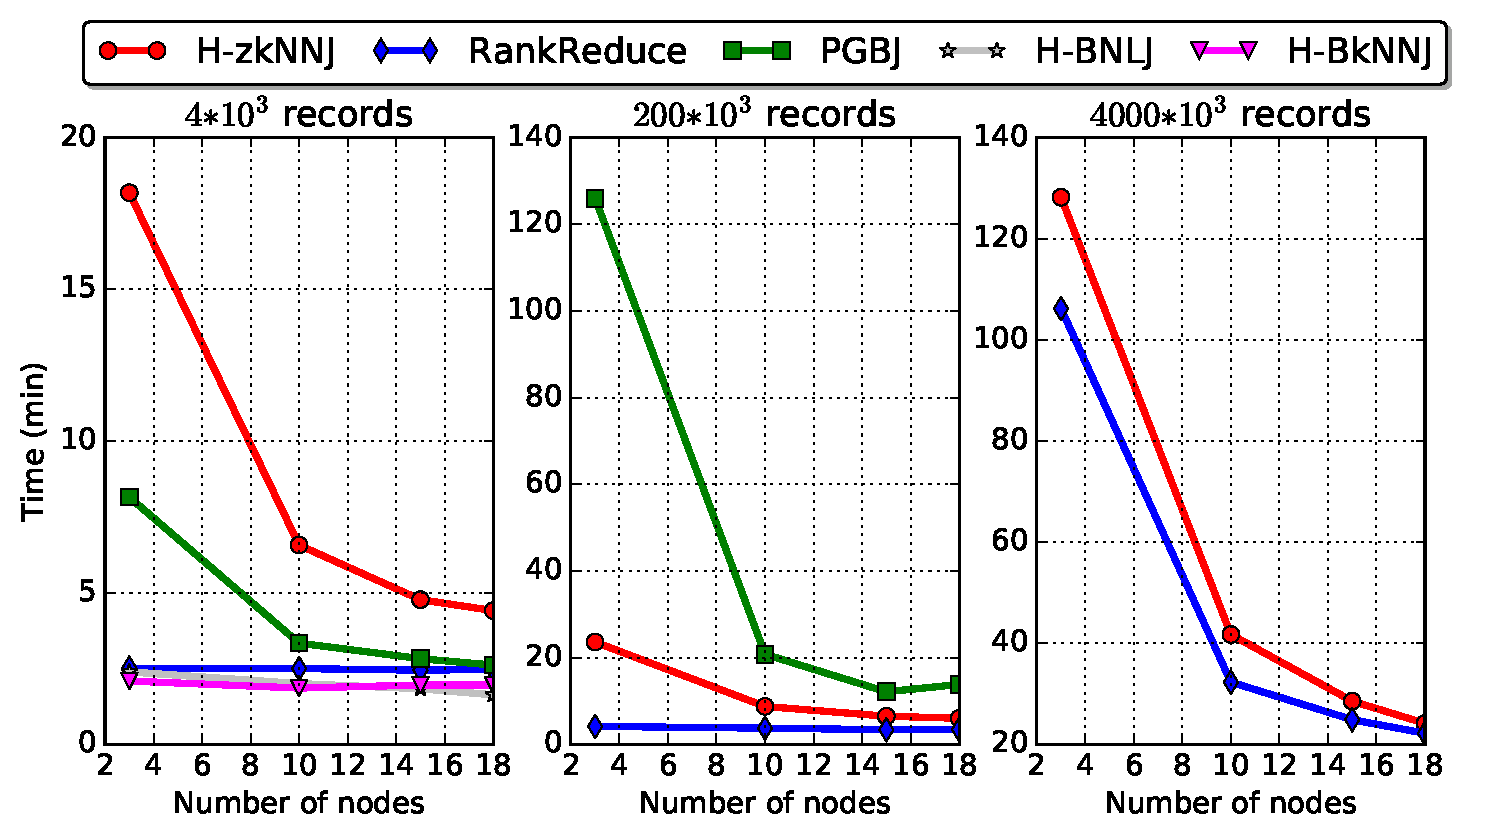
\includegraphics[width=0.5\textwidth]{img-perf/geo/data/nodes.pdf}
 \caption{Impact of the number of nodes on computing time  \label{fig:geo_data_nodes}}
\end{figure}

Figure~\ref{fig:geo_data_nodes} shows that the number of nodes used is strongly related to computing time. Increasing the 
number of nodes is almost always beneficial, especially for large datasets. 

%( for h-bknnj  -see section \TODO{5} -). 

%For all data sizes, after a certain threshold, adding new nodes has a negligible impact. We can consider the number of nodes before this stage as the best compromise between speedup and used resources.\\
%One can notice that, for RankReduce, the number of nodes decreases the time but it's significant just from a big dataset.\\

%\textit{From here, the performances are done on 20 nodes, 1 slot by node. the number of nearest neighbours equals to 20.}
%\\
%From here, all presented evaluations are executed using 20 nodes\footnote{Each node is set with a single Hadoop slot.}, and $k$ is set to 20 as well.
        
        
\subsubsection{Impact of k}
The number $k$ of requested nearest neighbours can have a significant impact on the performance of some of the kNN 
algorithms. We experimented on a dataset of $(200*10^{5})$ \TODO{Lea: can you check, that's a lot compared to previous run, 
especially for H-BNLJ} data, with  $k$ varying from 2 to 512. We measured computing time, disk usage, and accuracy, as shown in figure~\ref{fig:geo_k}.

%As already happened in previous evaluations, we display only the first values of H-BNLJ, as this algorithms takes too long 
%to complete. It certainly cannot compete with the other algorithms in this case.

For RankReduce, increasing $k$ has a negative impact on the accuracy which sharply declines when $K\geq 6$. The reason of 
this drop is that the window parameter of RankReduce remains unchanged for all the experimented $k$. The window parameter 
was empirically set for the first $k$ we experimented, so it was well-adapted for the first values of $k$, but less and 
less adapted as $k$ increased. This means that changing a parameter when using RankReduce should always lead to an 
empirical readaptation of the LSH parameters too maintain good accuracy. 
  
For H-zkNNj, the biggest impact of increasing $k$ is on the computing time. Although the disk usage starts high, it gets
lower as $k$ increases. Replication of data increases in order to find the required number of neighbours. Due to this fact, the computing time using H-zkNNj increases exponentially. \TODO{Lea: on Figure (b) zkNNJ has a low disk usage}.

However, for PGBJ, replication of data occurs independently of the number of selected neighbours. Thus, increasing $k$ has 
a small impact on this algorithm, both in computing time and space requirements.       
        
\subsection{Image Feature Descriptors dataset}
We now investigate whether the dimension of input data has a large impact on the kNN algorithms. Images feature descriptors 
are known to be high dimensional data. We chose to use compute the descriptors with SURF, which produces data
in dimension 128 (\TODO{Lea: check?}). \TODO{ We need more informations like number of descriptors per image, size...}
Results are shown in Figure~\ref{fig:surf_exp} and we omit H-BkNNJ as it could not process the data in reasonable time.
\TODO{Lea: How can execution time be that low, 3-6 seconds?!}
For H-zkNNJ \TODO{Lea: where is H-zkNNJ on the figure?!}, the accuracy drops  below 50 percent, because of the use 
of space filling curves, as explained in section \ref{z-value}. 

\subsubsection{Impact of the size of input data}       
In Figure~\ref{fig:surf_data}, we can see the behaviour of the three considered algorithms when varying the size of input 
data, in number of records. Computing time increases exponentially for PGBJ and H-BNLJ whereas RankReduce sees a linear 
increase. It cannot however reach more than 60\% accuracy.

\subsubsection{Impact of the number of nodes}
The only common with the previous dataset is that increasing the number of nodes to process the computation is beneficial
as it decreases computation time as shown in Figure~\ref{fig:surf_nodes}.
The partitioning in H-BNLJ depends on the number of nodes and, as a consequence, we can see that some values such as 30 gives much better performance than others \TODO{Lesquels ? quelle est la formule magique ?}. 
      
\subsubsection{Impact of $k$}    
Finally, Figure~\ref{fig:surf_k} shows the impact of the number of selected nearest neighbours on the computing time and 
the accuracy. For H-BNLJ and PGBJ, the computing time increases exponentially for low values of $k$. \TODO{relation avec le 
geo dataset} For RankReduce, the computing time is controlled with the increase of $k$ but at the expanse of a wretched 
accuracy. The last experimental case suffers from an accuracy of 20\%, which can hardly be satisfactory. The problem comes 
again from the static window parameter of the LSH method. The only way to keep an acceptable accuracy is to empirically 
compute the LSH parameters needed for this particular configuration.


\subsection{Dimensional or dataset dependent?}
In this section, we focus on the characteristics of input data instead of the characteristics of the algorithm, to explore in which extent the nature of data impact the performance of the algorithms. For that, we take several dataset from an online data bank\footnote{\url{https://archive.ics.uci.edu/ml/datasets.html}}. All dataset have data in different dimensions. for this set of experiments, we fix $k$ as to be equal to 20.

 \begin{figure}[!h]
 \centering
 \centering
		\begin{subfigure}[b]{0.25\textwidth}
                 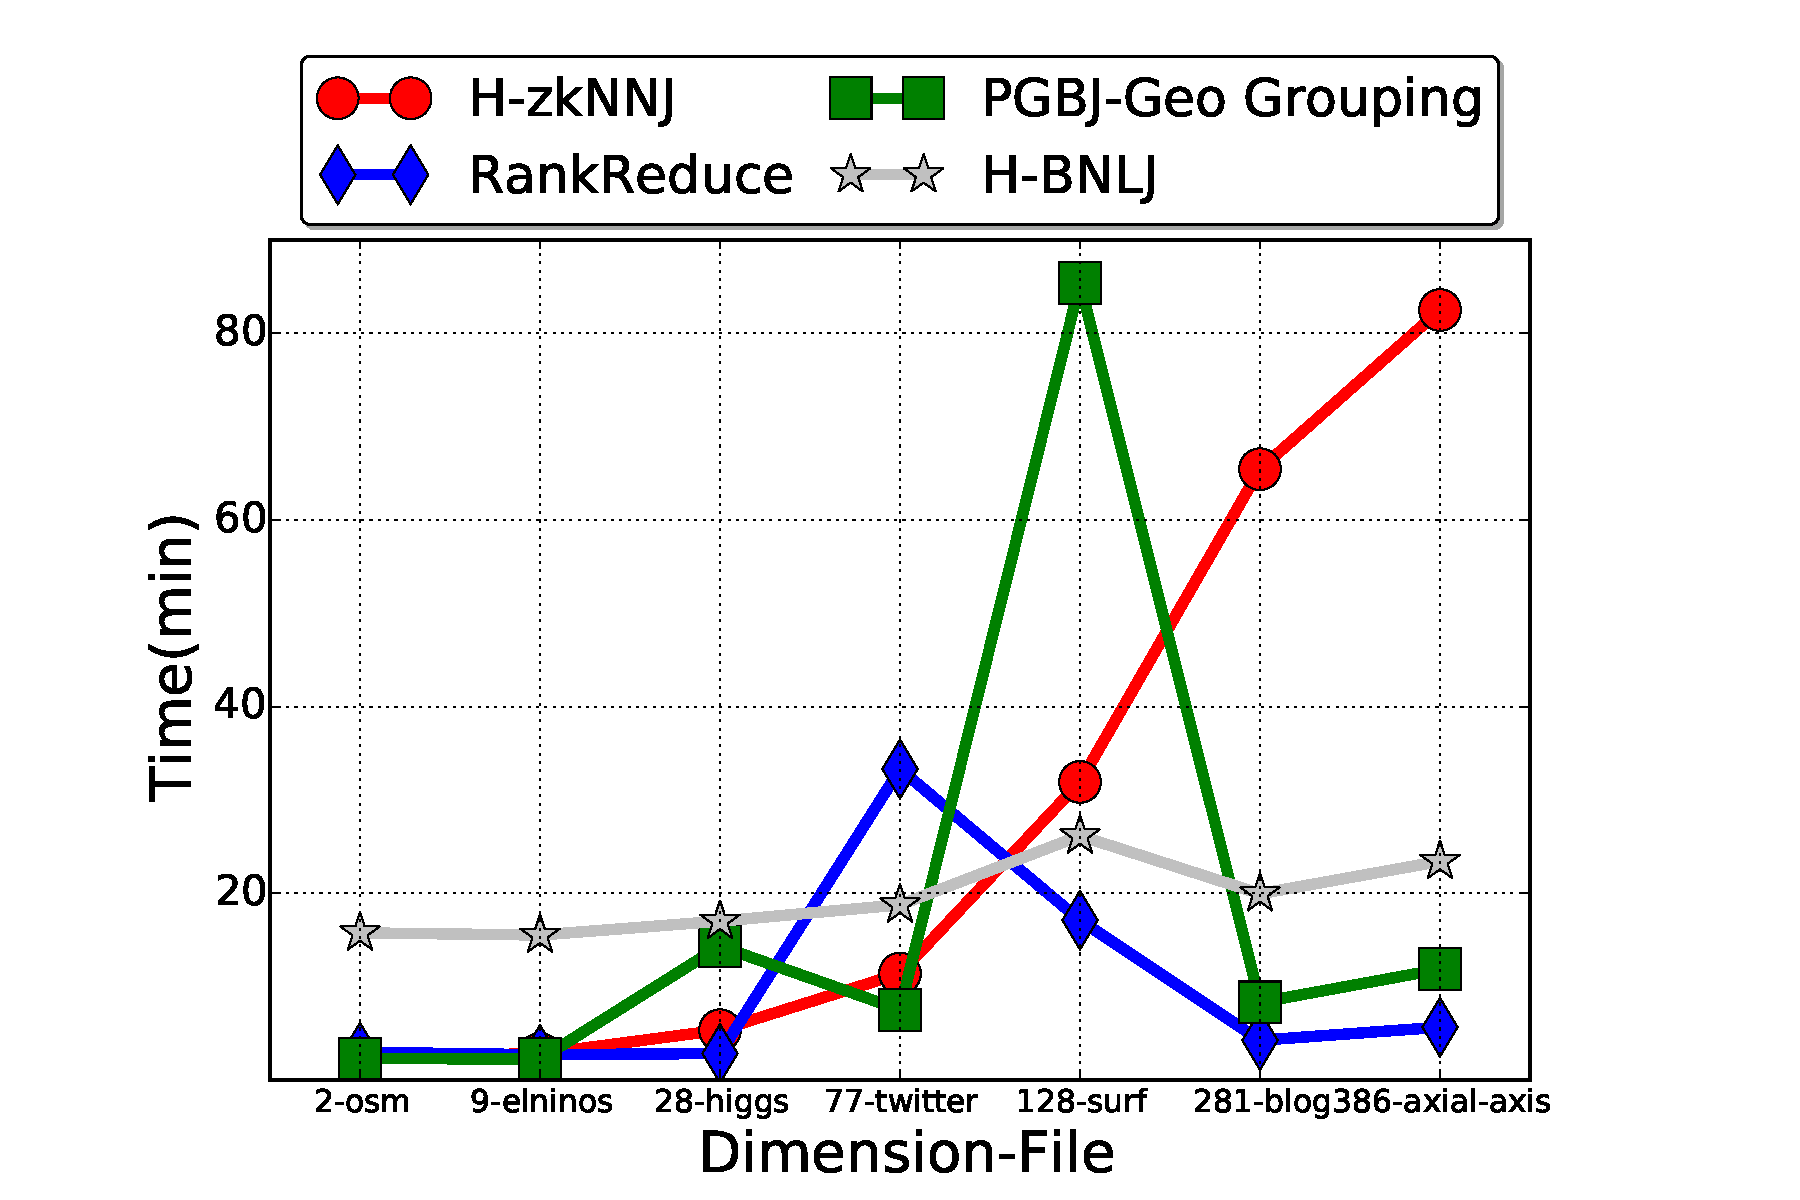
\includegraphics[width=\textwidth]{img-perf/dim/datasettime.pdf} 
                \caption{time}
                \label{dim_time}
        \end{subfigure}%
        \begin{subfigure}[b]{0.25\textwidth}
                 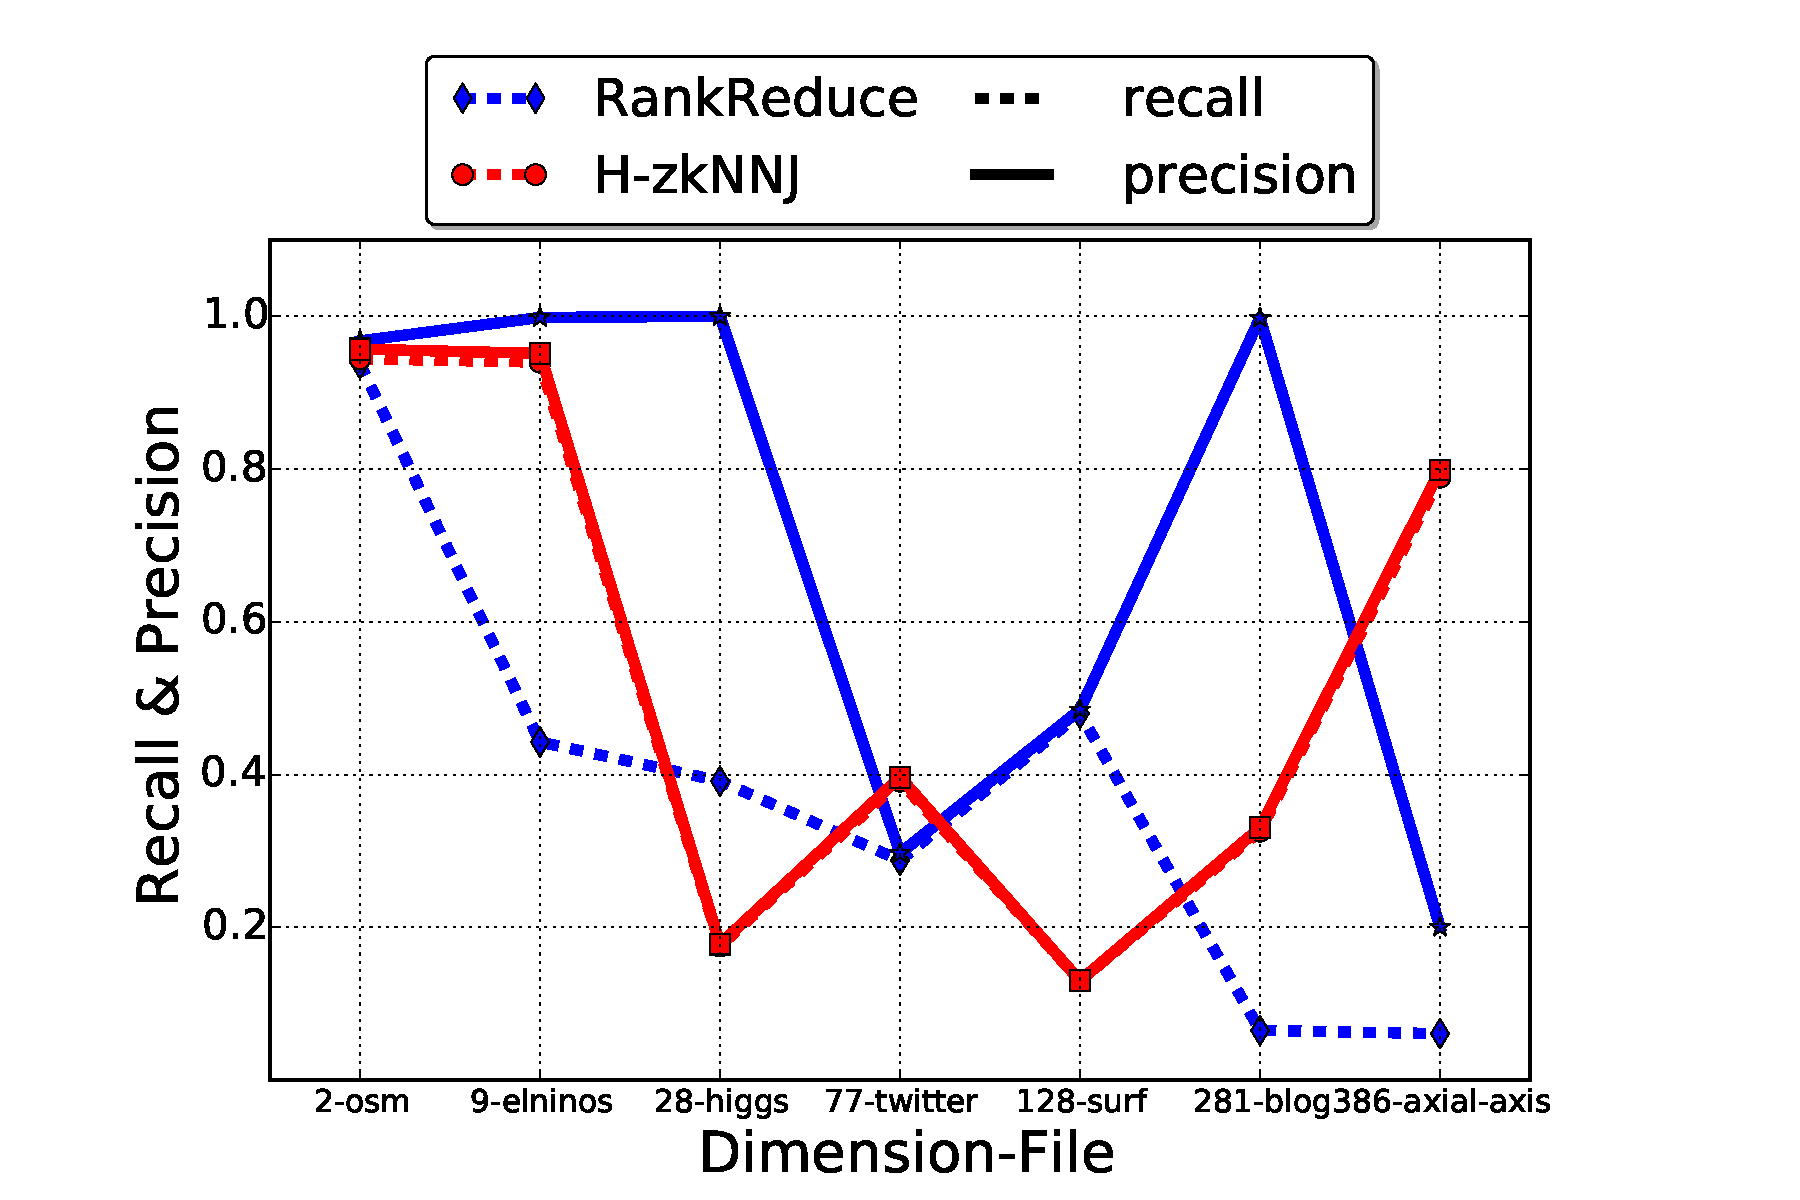
\includegraphics[width=\textwidth]{img-perf/dim/datasetacc.pdf} 
                \caption{accuracy}
                \label{dim_acc}
        \end{subfigure}
         \caption{impact of dimension with different dataset}
          \label{fig:dim}
\end{figure}

Figure \ref{fig:dim} displays the computing time of 5 different dataset with increasing dimensions. For most algorithms, results evolve smoothly, which suggests that the nature of data does not really impact the algorithm. However for PGBJ, the connection between dimension and computing time is not evident, because it first rises and then decreases for the highest experimented dimension. It seems to be due to the grouping method involved in PGBJ partitioning.
To confirm that it is the dimension that triggers this phenomenon \TODO{It is contradictory with the next result}, and not the nature of data, we set up a  fake dataset in which different dimensions are used and for which all data have equal distances. 
%We see,\ref{fig:dim}, that dimension deals on z-value's behaviour.\\
%The behaviour of Voronoi is strange. Already, we are tested with greedy and the time to compute the grouping is been too long and no efficient. Indeed,Voronoi depends of dataset to create its cells and greedy bounds the replication. due to this fact all cells are the replicas of all cells and greedy becomes no efficient.\\
%To confirm that it's just the dimension and not the different dataset that product this phenomenon, we create some file with different dimension where all data are to equals-distance.

\begin{figure}[!h]
 \centering
 \centering
		\begin{subfigure}[b]{0.25\textwidth}
                 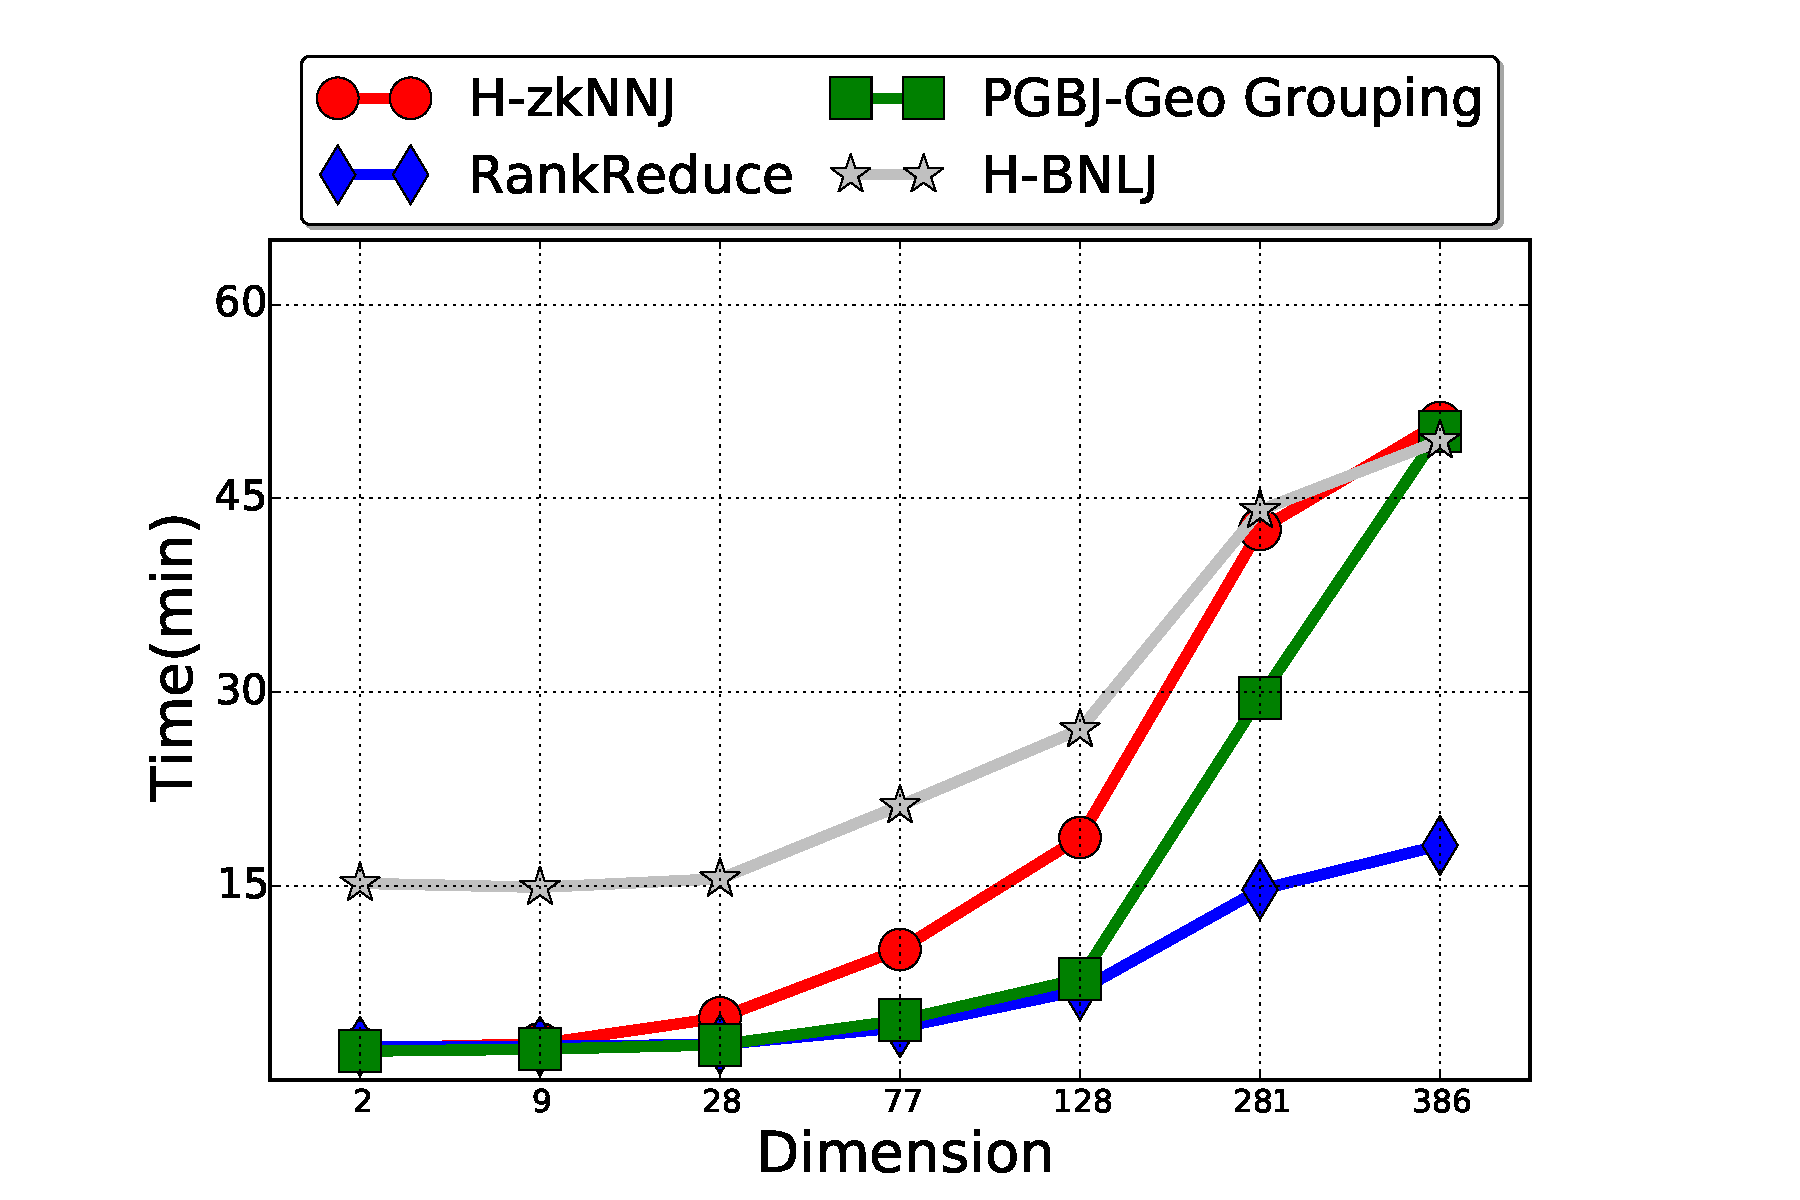
\includegraphics[width=\textwidth]{img-perf/dim/randtime.pdf} 
                \caption{time}
                \label{dim_rand_time}
        \end{subfigure}%
        \begin{subfigure}[b]{0.25\textwidth}
                 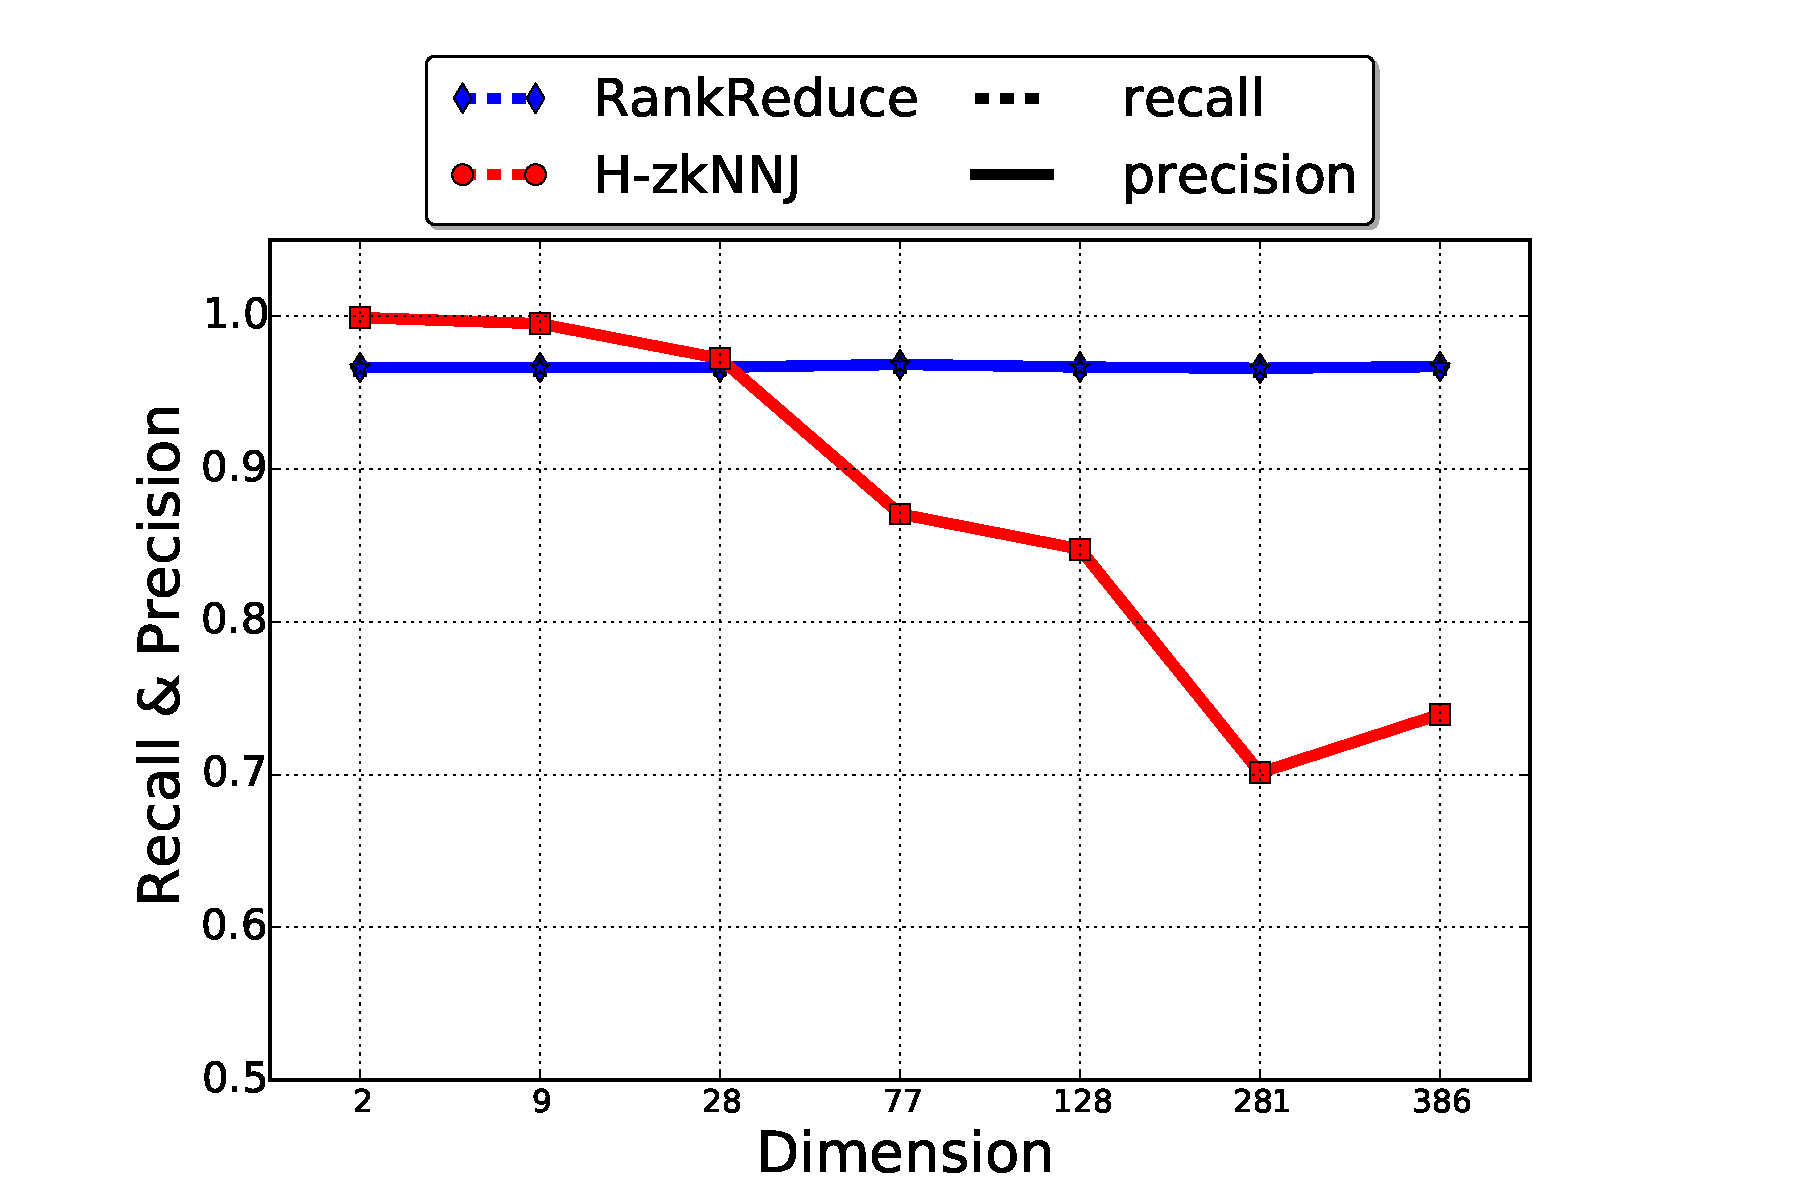
\includegraphics[width=\textwidth]{img-perf/dim/randacc.pdf} 
                \caption{accuracy}
                \label{dim_rand_acc}
        \end{subfigure}
         \caption{impact of dimension with random dataset}
          \label{fig:dim_rand}
\end{figure}
The result of this new setting can be seen on figure \ref{fig:dim_rand}.
All algorithms behave then regularly which means that the nature of the dataset has an impact on the performance of PGBJ. Nevertheless, it also means that the other algorithms behave in the same way as previously: those algorithms are indeed impacted by the dimension of the input data, and the most impacted algorithm is H-zkNNJ, in spite of a good accuracy for this approximate algorithm.
Another aspect of the results is thus that it is not necessarily the dimension of input data that impact the accuracy of H-zkNNJ, but the nature of the dataset, whereas the accuracy of H-LSH is mainly impacted by the crucial parameters of LSH.

%We see that in spite of good accuracy Z-VALUE behaves in the same way. By consequence the dimension increases the time of Z-VALUE.\\
%We see a other aspect, it isn't necessary the dimension that influences the accuracy of Z-VALUE but rather its 	dataset. And by this fact, Z-VALUE is efficient for all dataset...
%For LSH the accuracy decreases. and we have to set the parameter. 
%J'ai une perf avec 4 dataset de dimension 2 on on voit different comportement mais pas trop...
 
 
\subsection{The problems of each algorithm}
In this section, we review the difficulties of each algorithms, that might lead to a selection by elimination of the best algorithm to choose for a particular use case.
\subsubsection{H-BkNNJ}
%HBKNNJ
\begin{figure}[!h]
\centering
                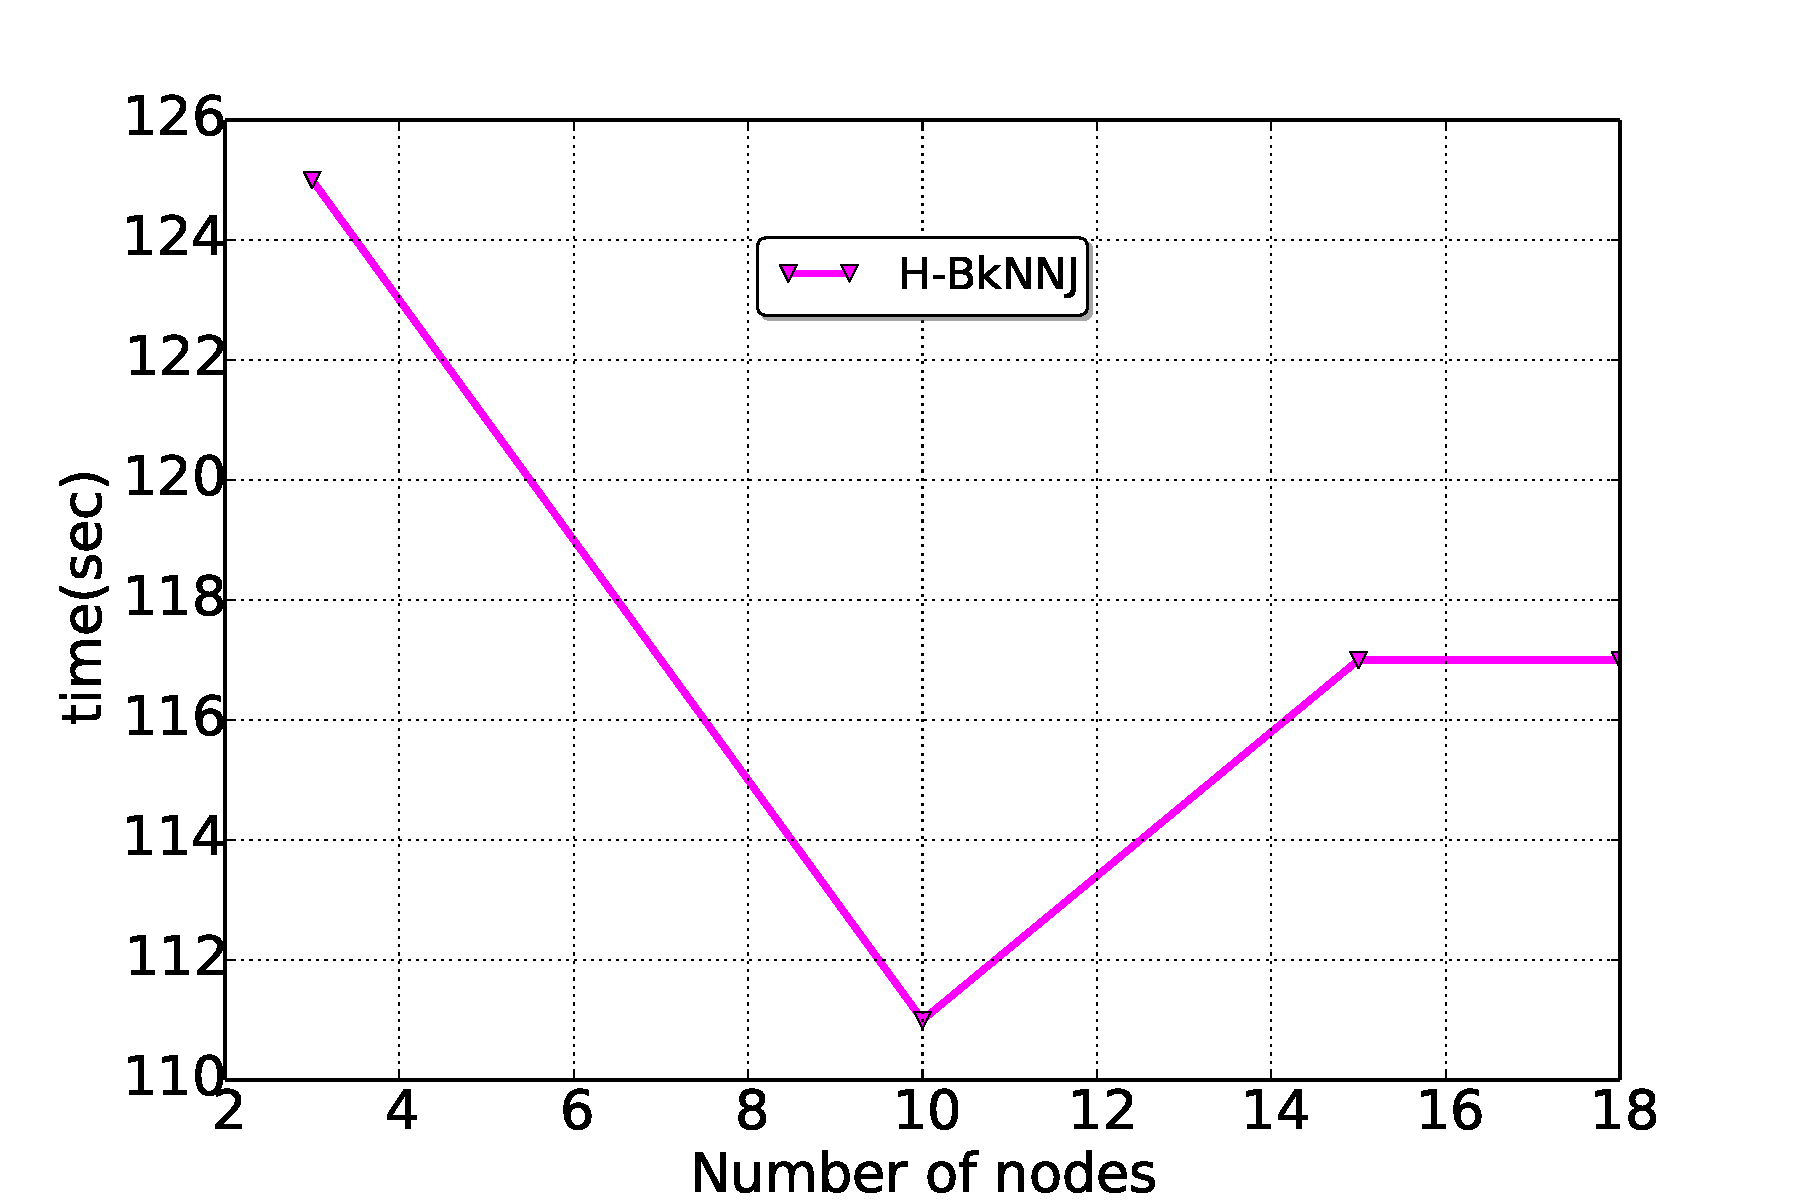
\includegraphics[width=0.5\textwidth]{img-perf/perso/hbknnj/nodes.pdf}
 \caption{hbknnj - \#nodes}
 \label{hbknnj_exp}
\end{figure}
The main drawback of H-BkNNJ is that only the Map phase is parallel. In addition, the optimal parallelization is subtle in the sense that the optimal number of nodes to used is dependent on the size of an input split (the unit that will be given to a Map), as can be seen on figure~\ref{hbknnj_exp}. The optimal number of nodes to use is defined by  $=|\sum input size|/input split  size$. This algorithm does not scale with input data increase but might be the best to use for small dataset, in terms of easiness of development.
%Only Map phase is parallel. The map phase split the input file in 64MB, so we can defined the optimal number of nodes $=|\sum inputfile|/64$. Only useful for some small data.

\subsubsection{H-BNLJ}
In H-BNLJ, both the Map and Reduce phase are parallelizable, but the optimal number of reducer is difficult to find. Figure~\ref{fig:hbnlj_reducer} shows some experimental values for this. It should minimize the quantity of calculation and optimize the parallelism at the same time. But this last point is challenging \TODO{resolve:}\ref{img-perf/perso/hbnlj/loadbalancing.png},
as it is mainly due to an imbalanced random distribution \TODO{resolve:}\ref{img-perf/perso/hbnlj/loadbalancing.png}.
H-BNLJ replicates all data the same number of time (number of partition) and compute all pairs, it thus does not gracefully scale even if it is slightly better than H-BkNNJ.
%choice nb reducers/number partitions
\begin{figure}[!h]
\centering
                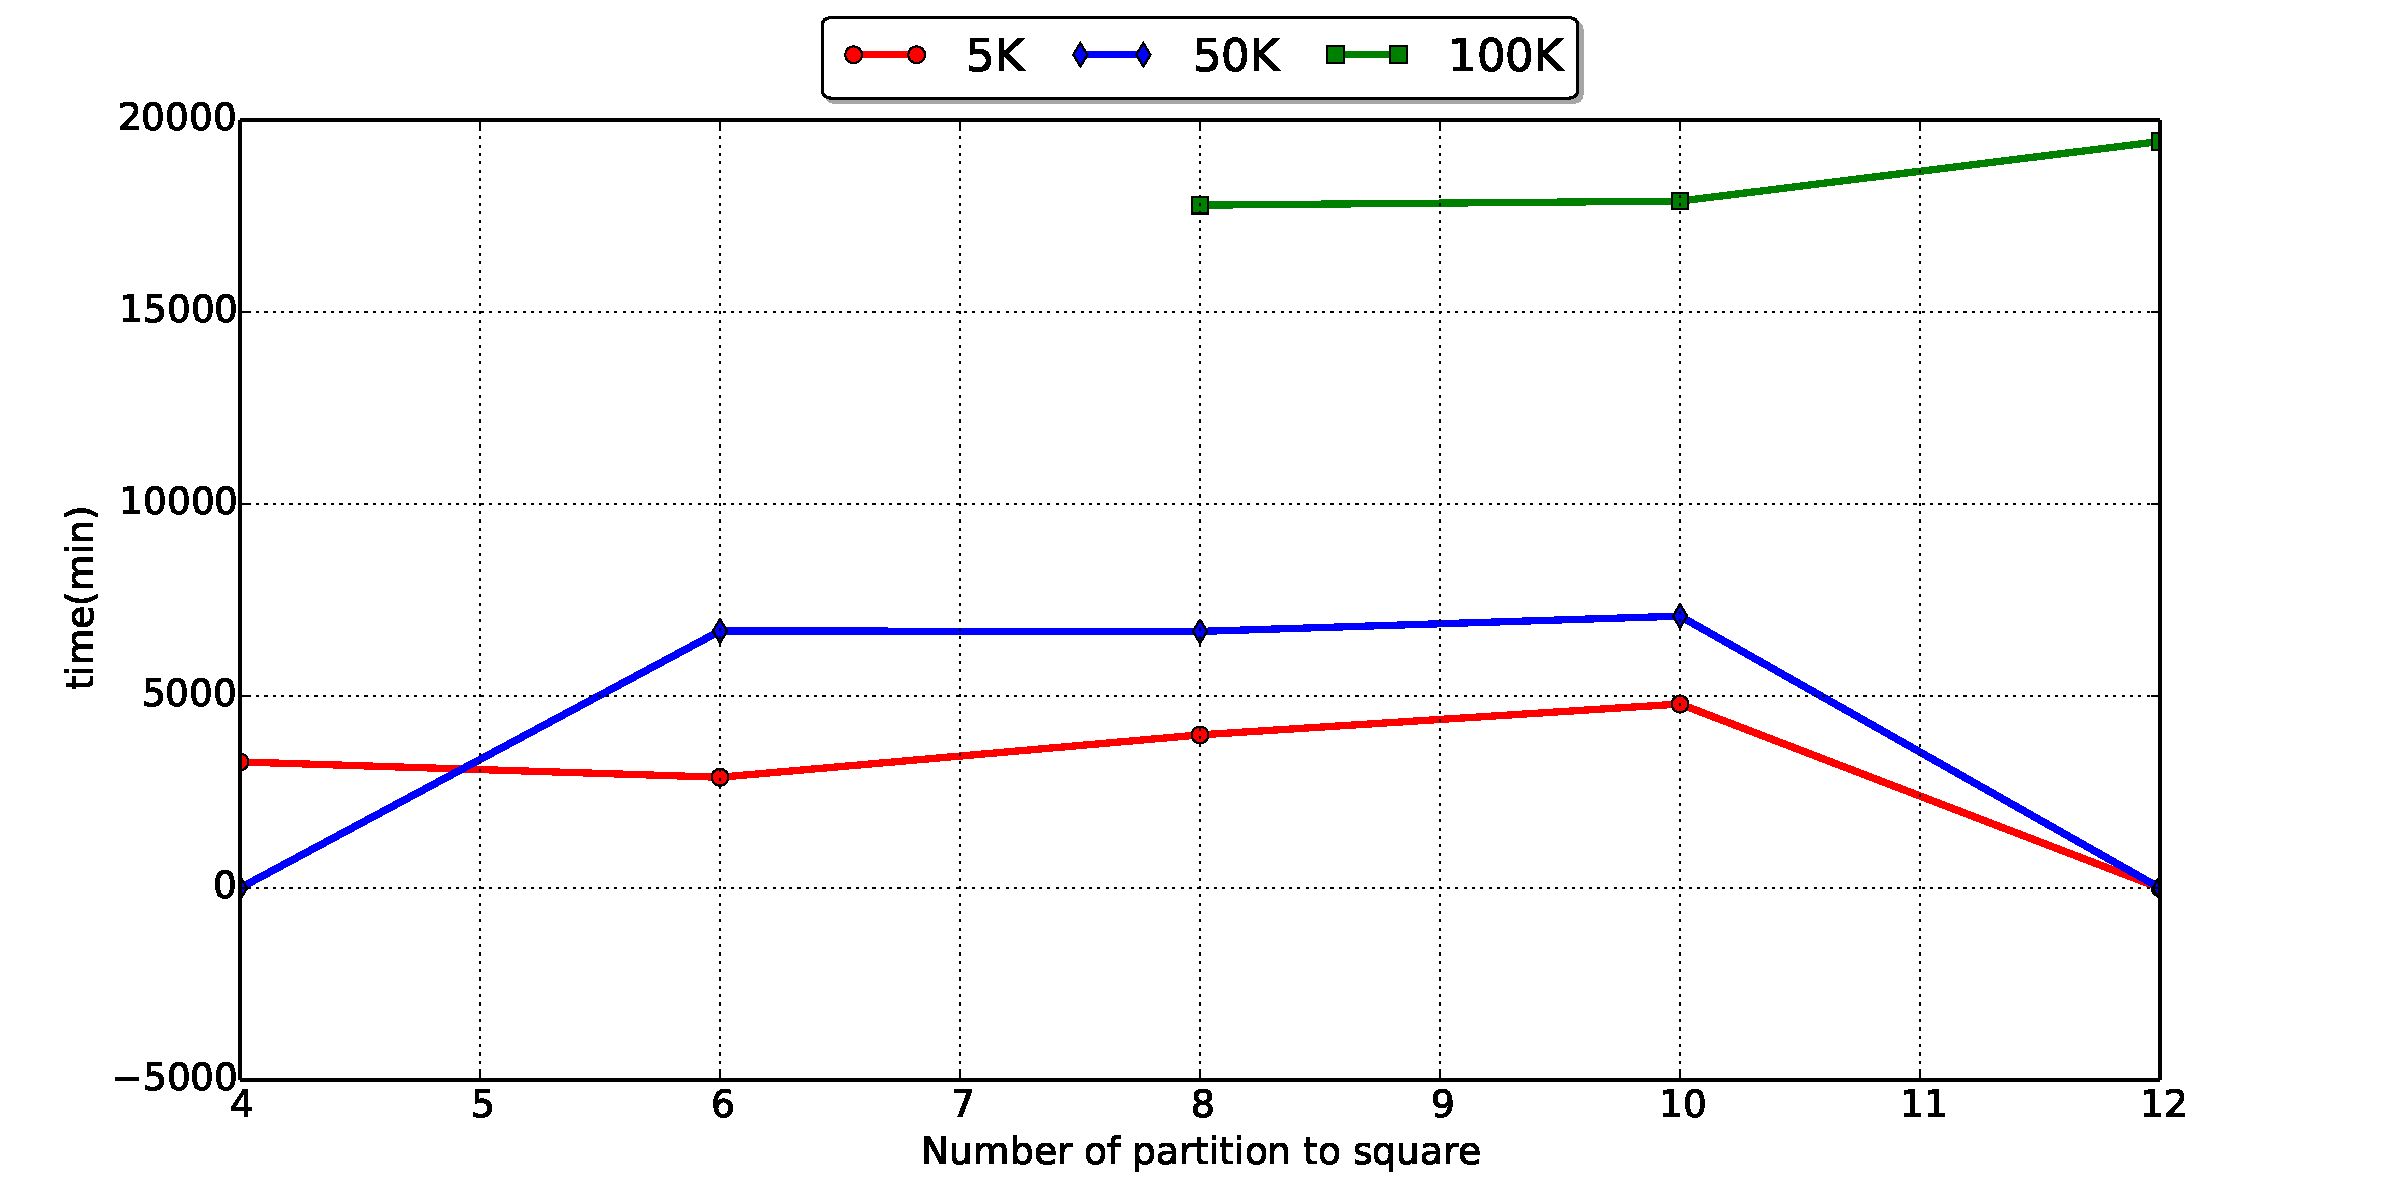
\includegraphics[width=0.5\textwidth]{img-perf/perso/hbnlj/reducer.pdf}
                \caption{H-BNLJ - \#reducers}
                \label{fig:hbnlj_reducer}
\end{figure}


\subsubsection{PGBJ}
The main difficulty in PGBJ is that its preprocessing techniques are based on a sampling.
The performance of this algorithm thus depends on the quality of the sampling. The different preprocessing techniques proposed help having a good partitioning and thus having a good load balance.
%\textbf{Samples :} the risk of the samples, either not statistic or not the way we want.
 \begin{figure}[!h]
 \centering
 
 \begin{subfigure}[b]{0.28\textwidth}
                 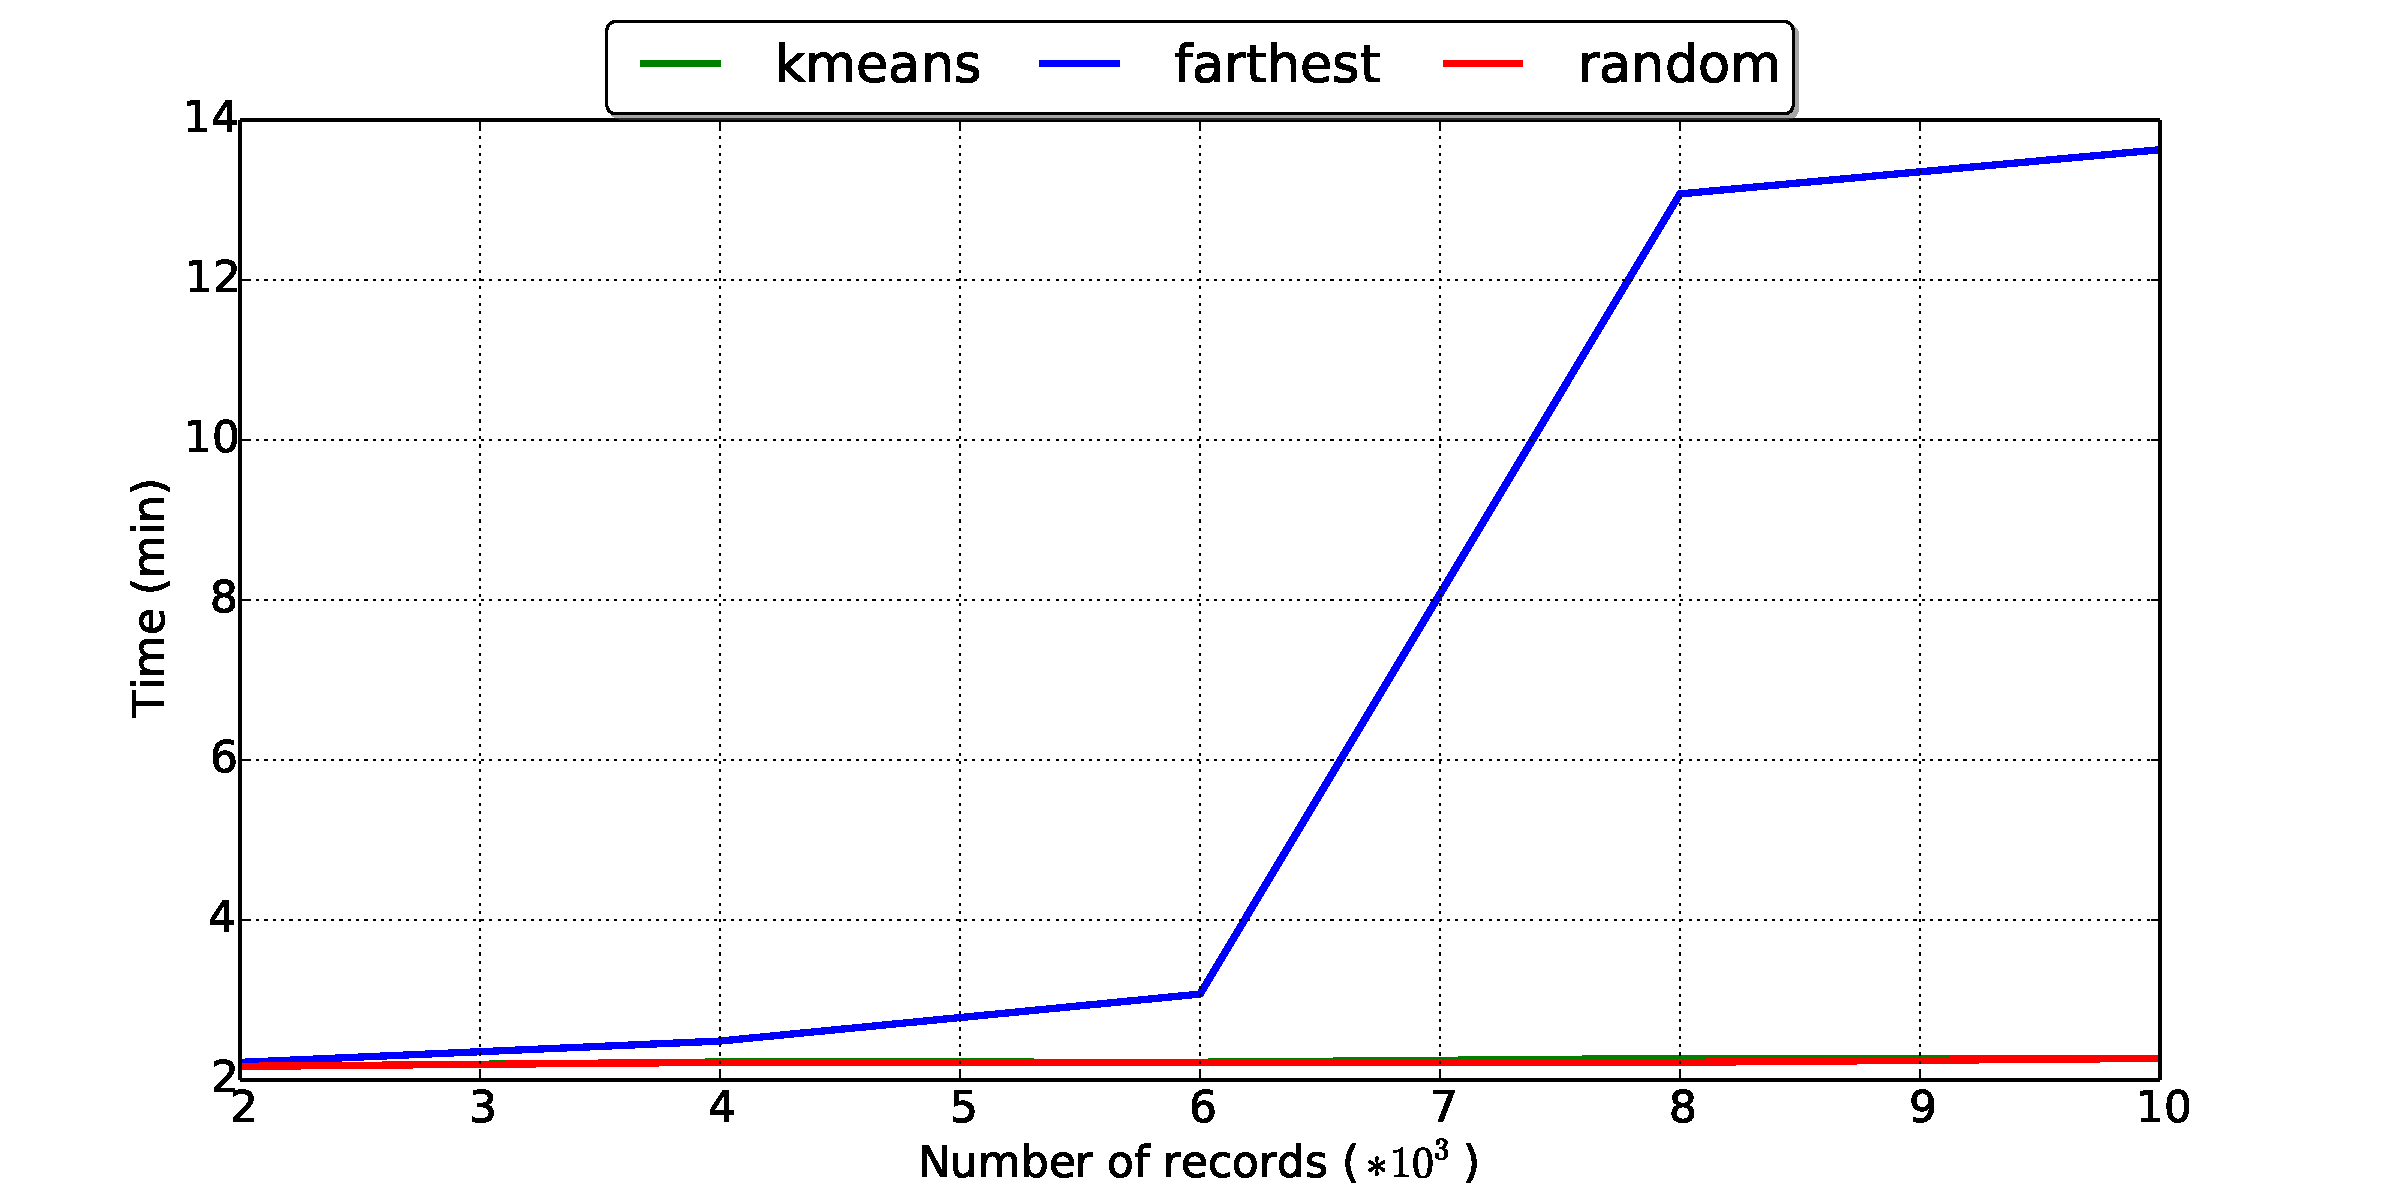
\includegraphics[width=\textwidth]{img-perf/perso/pgbj/sample.pdf} 
                \caption{Sampling}
                  \label{fig:pgbj_samples}
        \end{subfigure}%        
        \begin{subfigure}[b]{0.28\textwidth}
                 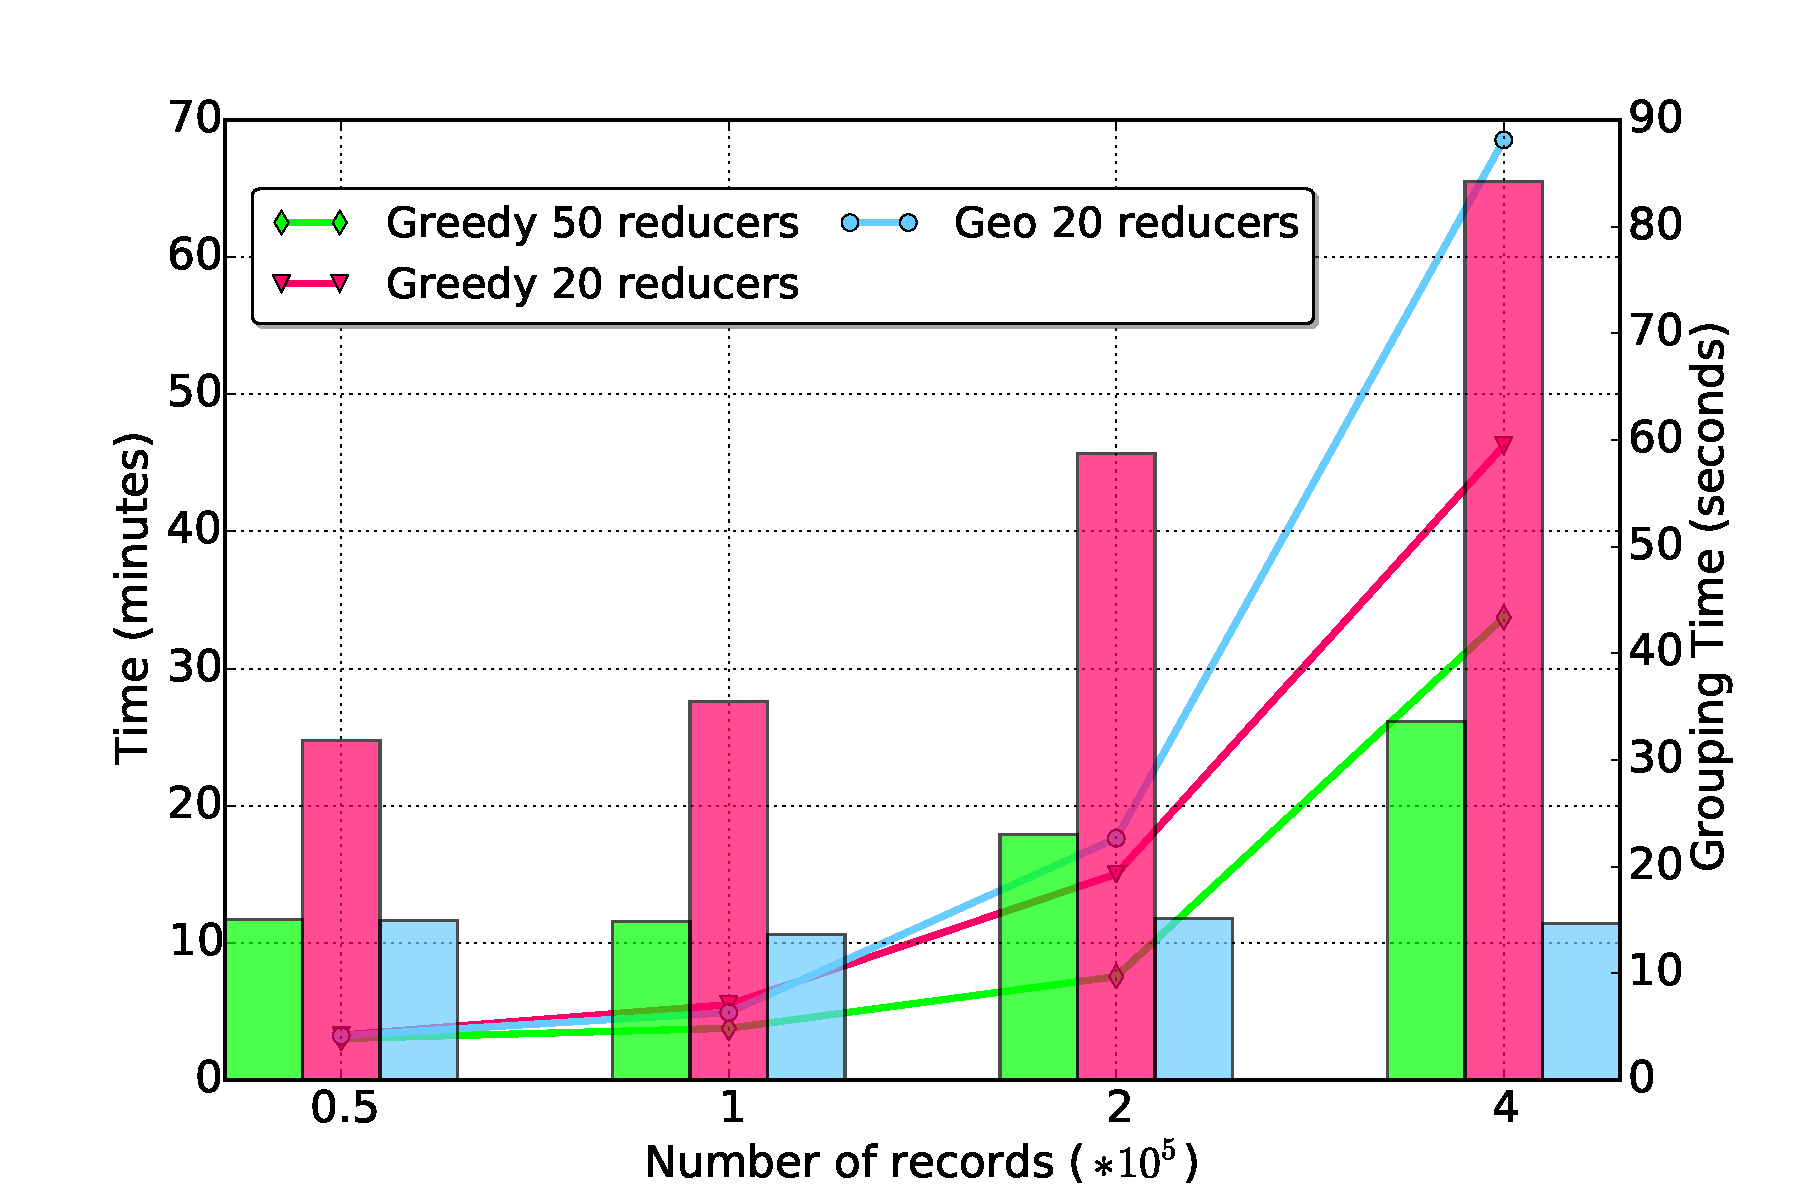
\includegraphics[width=\textwidth]{img-perf/perso/pgbj/strategy.pdf} 
                \caption{Grouping strategies}
                  \label{fig:pgbj_strategy}
                   \end{subfigure}
                  
                   \caption{PGBJ performance}
                  \label{fig:pgbj}
        \end{figure}
        
         In figure \ref{fig:pgbj_strategy}, we can see that the greedy grouping technique has a higher grouping time than the geo-grouping technique. But in the end, the global computing time using this technique is faster thanks to the good load balancing it leads to. Moreover, having a few more Reducers enables also a time gain.
        
        
\subsubsection{H-zkNNJ}\label{z-value}
H-zkNNJ is based on the method of Z space filling curve. This method transforms the space dimension into a one-dimensional space.
This reduction inevitably leads to information loss, and by consequence, the nature of the dataset, the dimension of data, and the size of the input data have a significant impact on the accuracy of this algorithm.
More specifically, this algorithm becomes biased if the distance between initial data is very scattered, and the more input data there are, the more difficult it is to draw the filling curve, as it is when data have high dimensions.
However, for a reasonable size of input data, and for low dimension data, H-zkNNJ is an efficient algorithm that may perform extremely fast and give acceptable results.
% But it stays one approximate method. And by consequence the good accuracy of Z-VALUE depends of the map result that depends of dataset initial. Therefore, the dataset \ref{fig:dataset}, the dimension  \ref{fig:dimension},and the number of data \ref{geo_data_accuracy} have a important impact on this accuracy. The first , if the distance between elements is very scattered. The second, because more  dimension is hight, more the reduction of dimension is approximate. The third, because more data mains more difficulties to draw the Z and thus to construct a good map.
%But for little dimension, Z-Value stays a algorithm quickly thanks to its reduction and its B-Tree to sort the data.

%dataset shift
\begin{figure}[!h]
\centering
                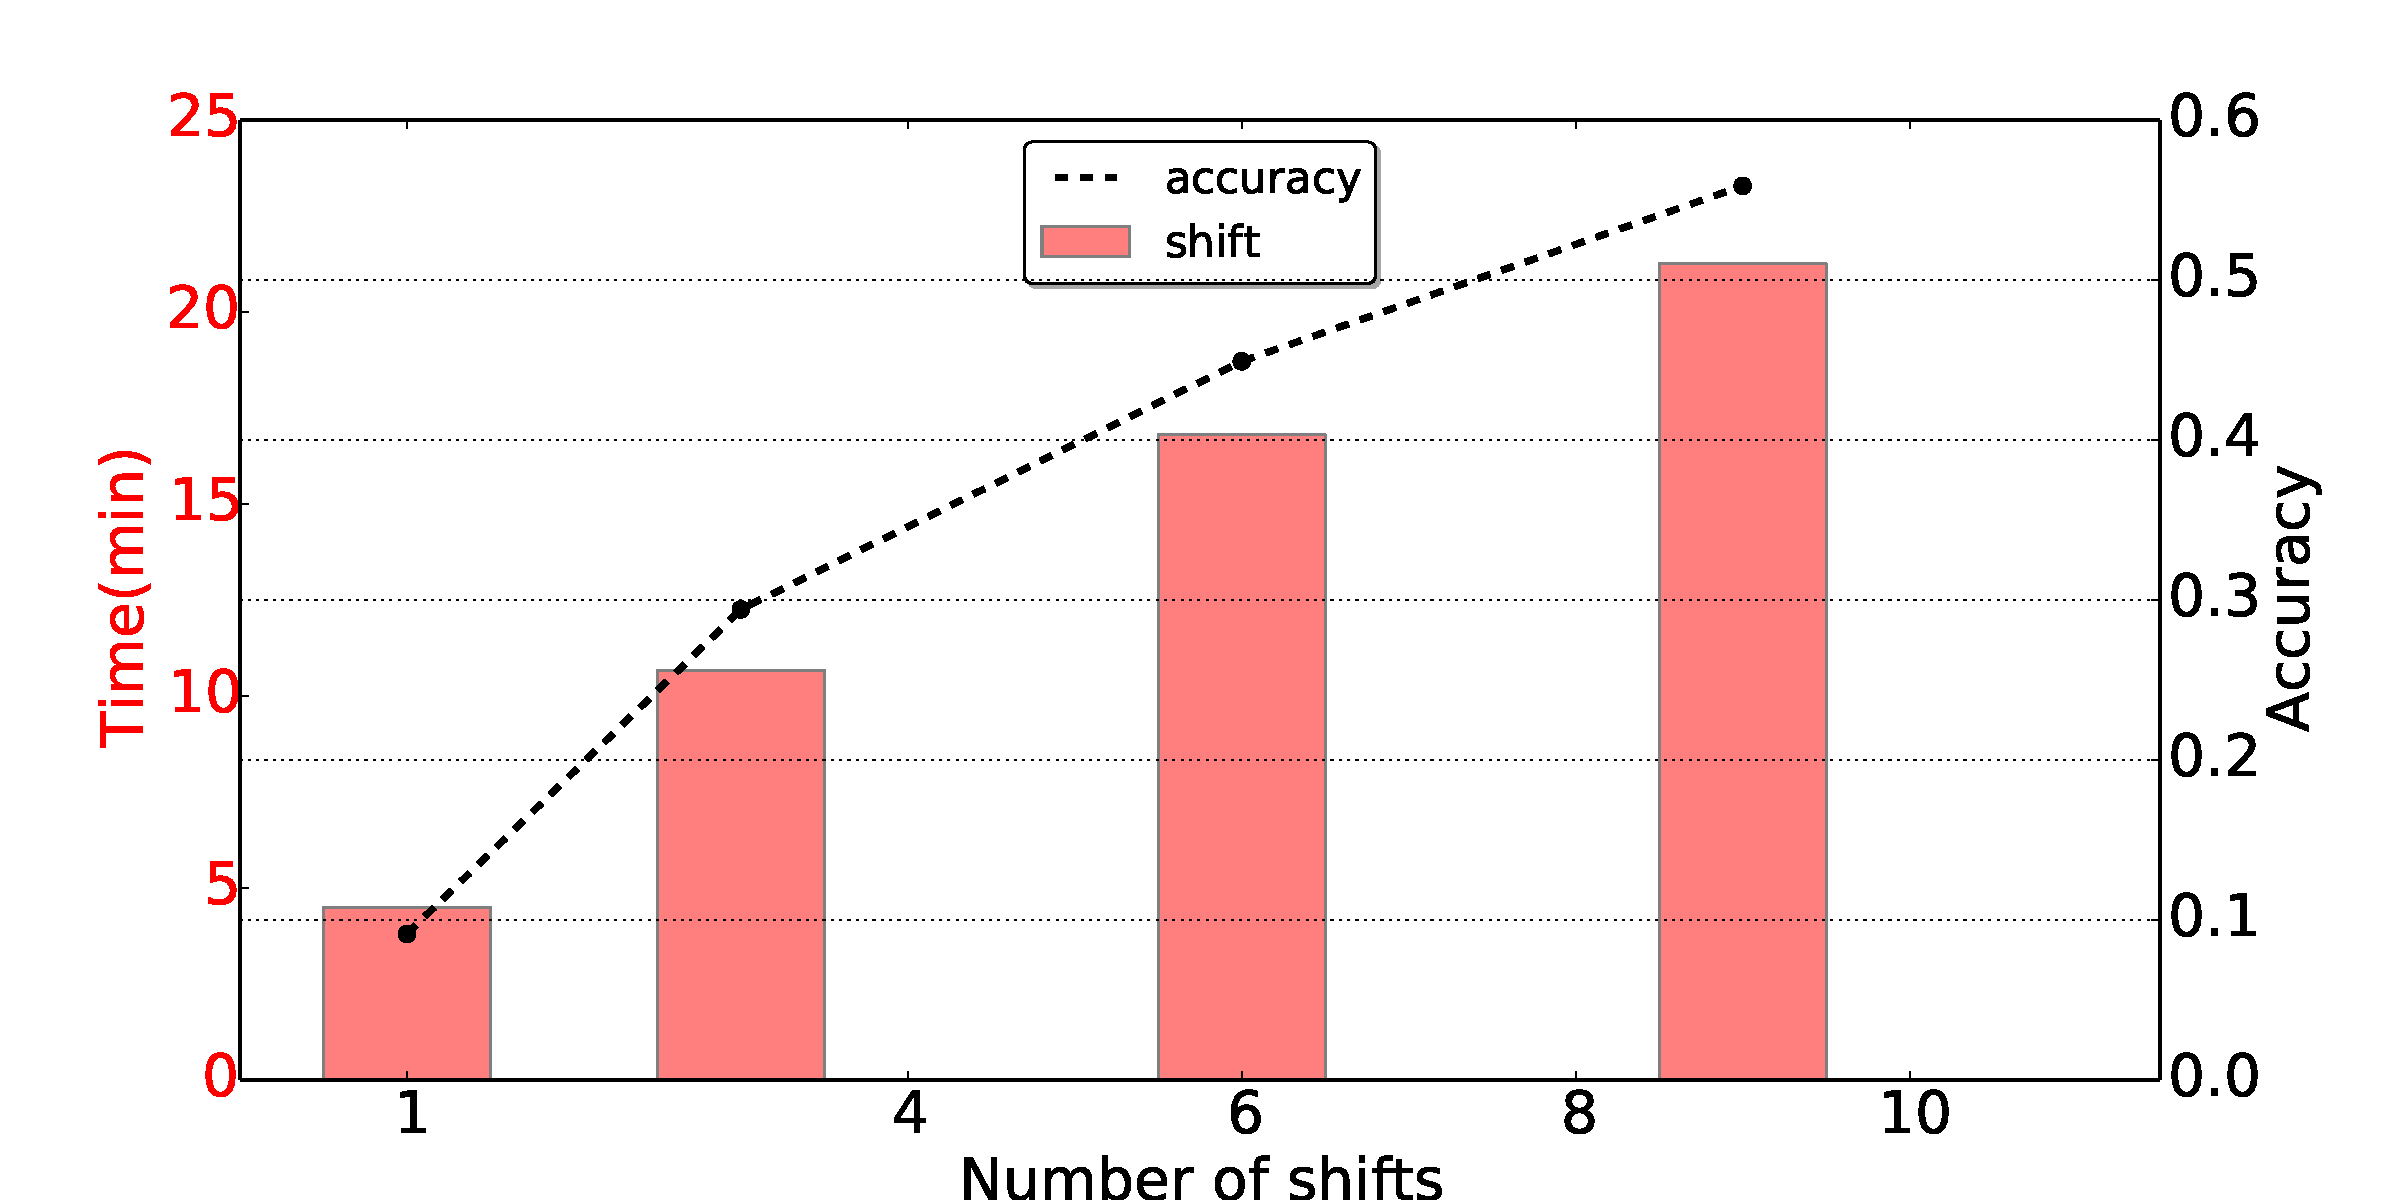
\includegraphics[width=0.3\textwidth]{img-perf/perso/hzknnj/shift.pdf}
                \caption{impact \#shift on surf dataset  }
                \label{fig:shift_dataset}
\end{figure}

\subsubsection{LSH}
H-LSH can be the outstanding algorithm with one prerequisite: having the goods parameters.
However finding the good parameters depends on the dataset itself, and by this means that the good parameter have to be decided experimentally. Nevertheless, studies can be found to choose acceptable parameters theoretically\TODO{mettre link http://www.cs.princeton.edu/cass/papers/cikm08.pdf }.
One might use a sample of its real data to extract the good LSH parameters to use for its dataset.
In figure \ref{fig:lsh_tunning_geo}, we see that having less buckets lead to a good accuracy but this does not fit the objective of improving the parallelism.
But having a small number of buckets doesn't impact a lot on accuracy though, it impacts only on computing time. Then, there must be a trade of between time and accuracy.
A special care must be taken when the dimension of data increases, because in this case the accuracy decreases, as shown in figure \ref{dim_rand_acc}, because the hash functions perform then worse.
One other drawback of H-LSH is that a certain number of copies must be used to have an acceptable accuracy, which has a constant impact on the required memory.


%Parameter Tuning.
%There are a lot of studies about tuning of lsh :
%\TODO{mettre link http://www.cs.princeton.edu/cass/papers/cikm08.pdf }.
%It 'is very difficult to find the good parameters for lsh because the parameters depend of dataset and thus the choice is empirical.
%In figure \ref{fig:lsh_tunning_geo}, we see that less bucket mains a good accuracy but it isn't our goal that is to improve the parallelism.
%But a little bit of bucket doesn't impact a lot on accuracy, only on time. We have to do an agreement between time and accuracy.
%While the dimension increases, the accuracy decreases, \ref{dim_rand_acc} because of hash function is less performance.
%And we have to add a number of copy (parameter L). \ref{fig:lsh_tunning_surf}
% 

 \begin{figure}[!h]
 \centering
		\begin{subfigure}[b]{0.25\textwidth}
                 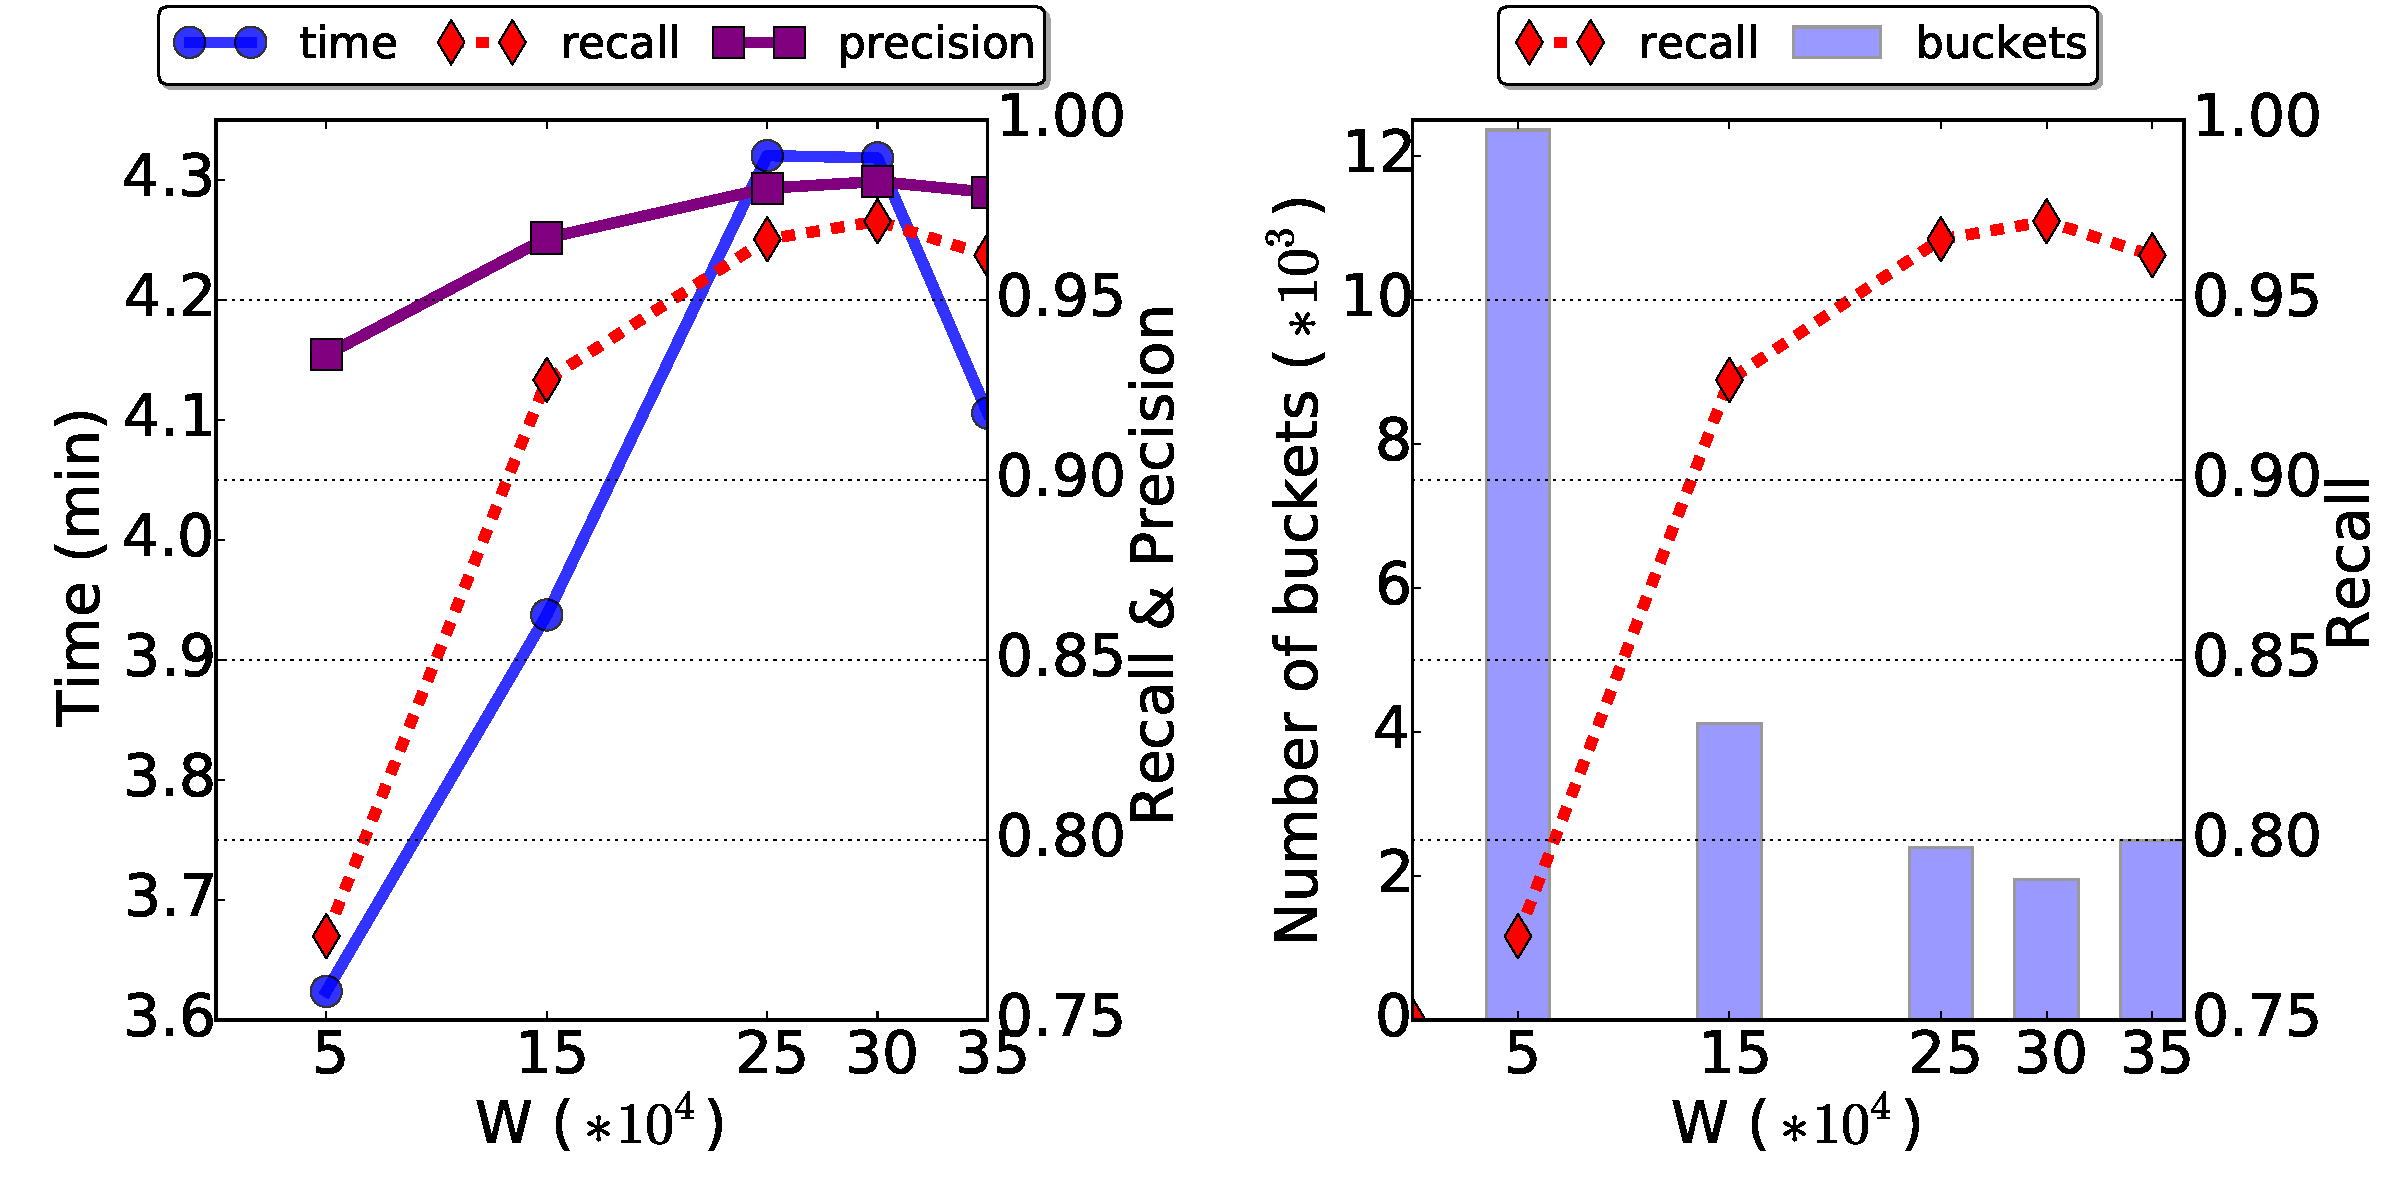
\includegraphics[width=\textwidth]{img-perf/perso/lsh/params_geo_time.pdf} 
                \caption{time}
                \label{fig:lsh_tunning_geo_time}
        \end{subfigure}%
		\begin{subfigure}[b]{0.25\textwidth}
                 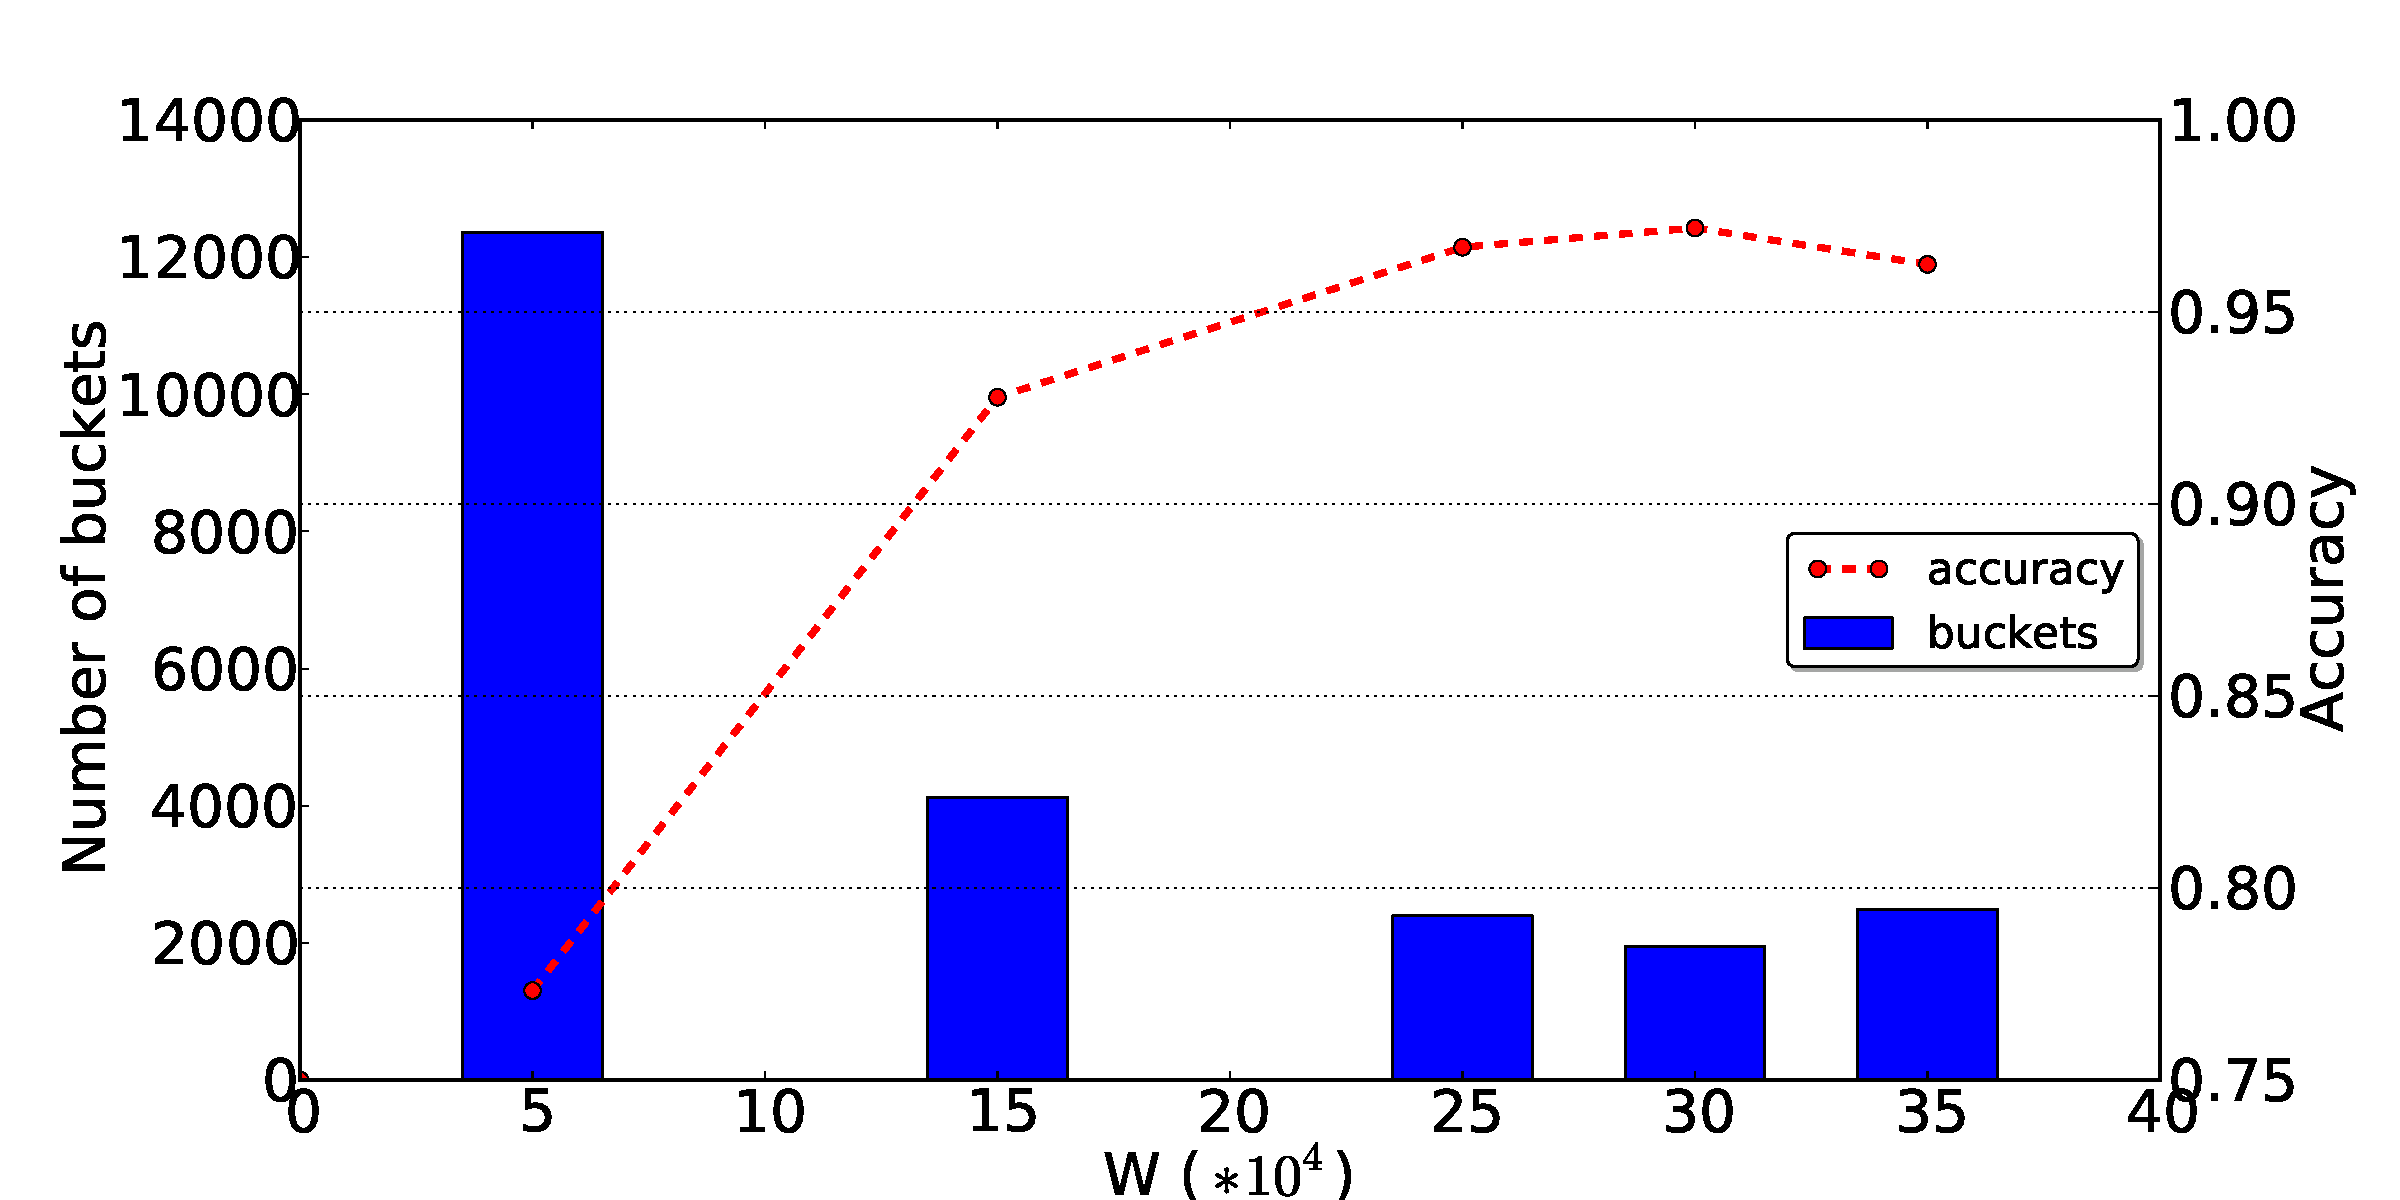
\includegraphics[width=\textwidth]{img-perf/perso/lsh/params_geo_acc.pdf} 
                \caption{accuracy}
                \label{fig:lsh_tunning_geo_acc}
        \end{subfigure}
         \caption{lsh tunning geo}
                \label{fig:lsh_tunning_geo}
\end{figure}

\TODO{Lea: verifie que les legendes L=..., M=... correspondent bien à la bonne courbe}
\begin{figure}[!h]
         \centering
       % \begin{subfigure}[b]{0.25\textwidth}
                 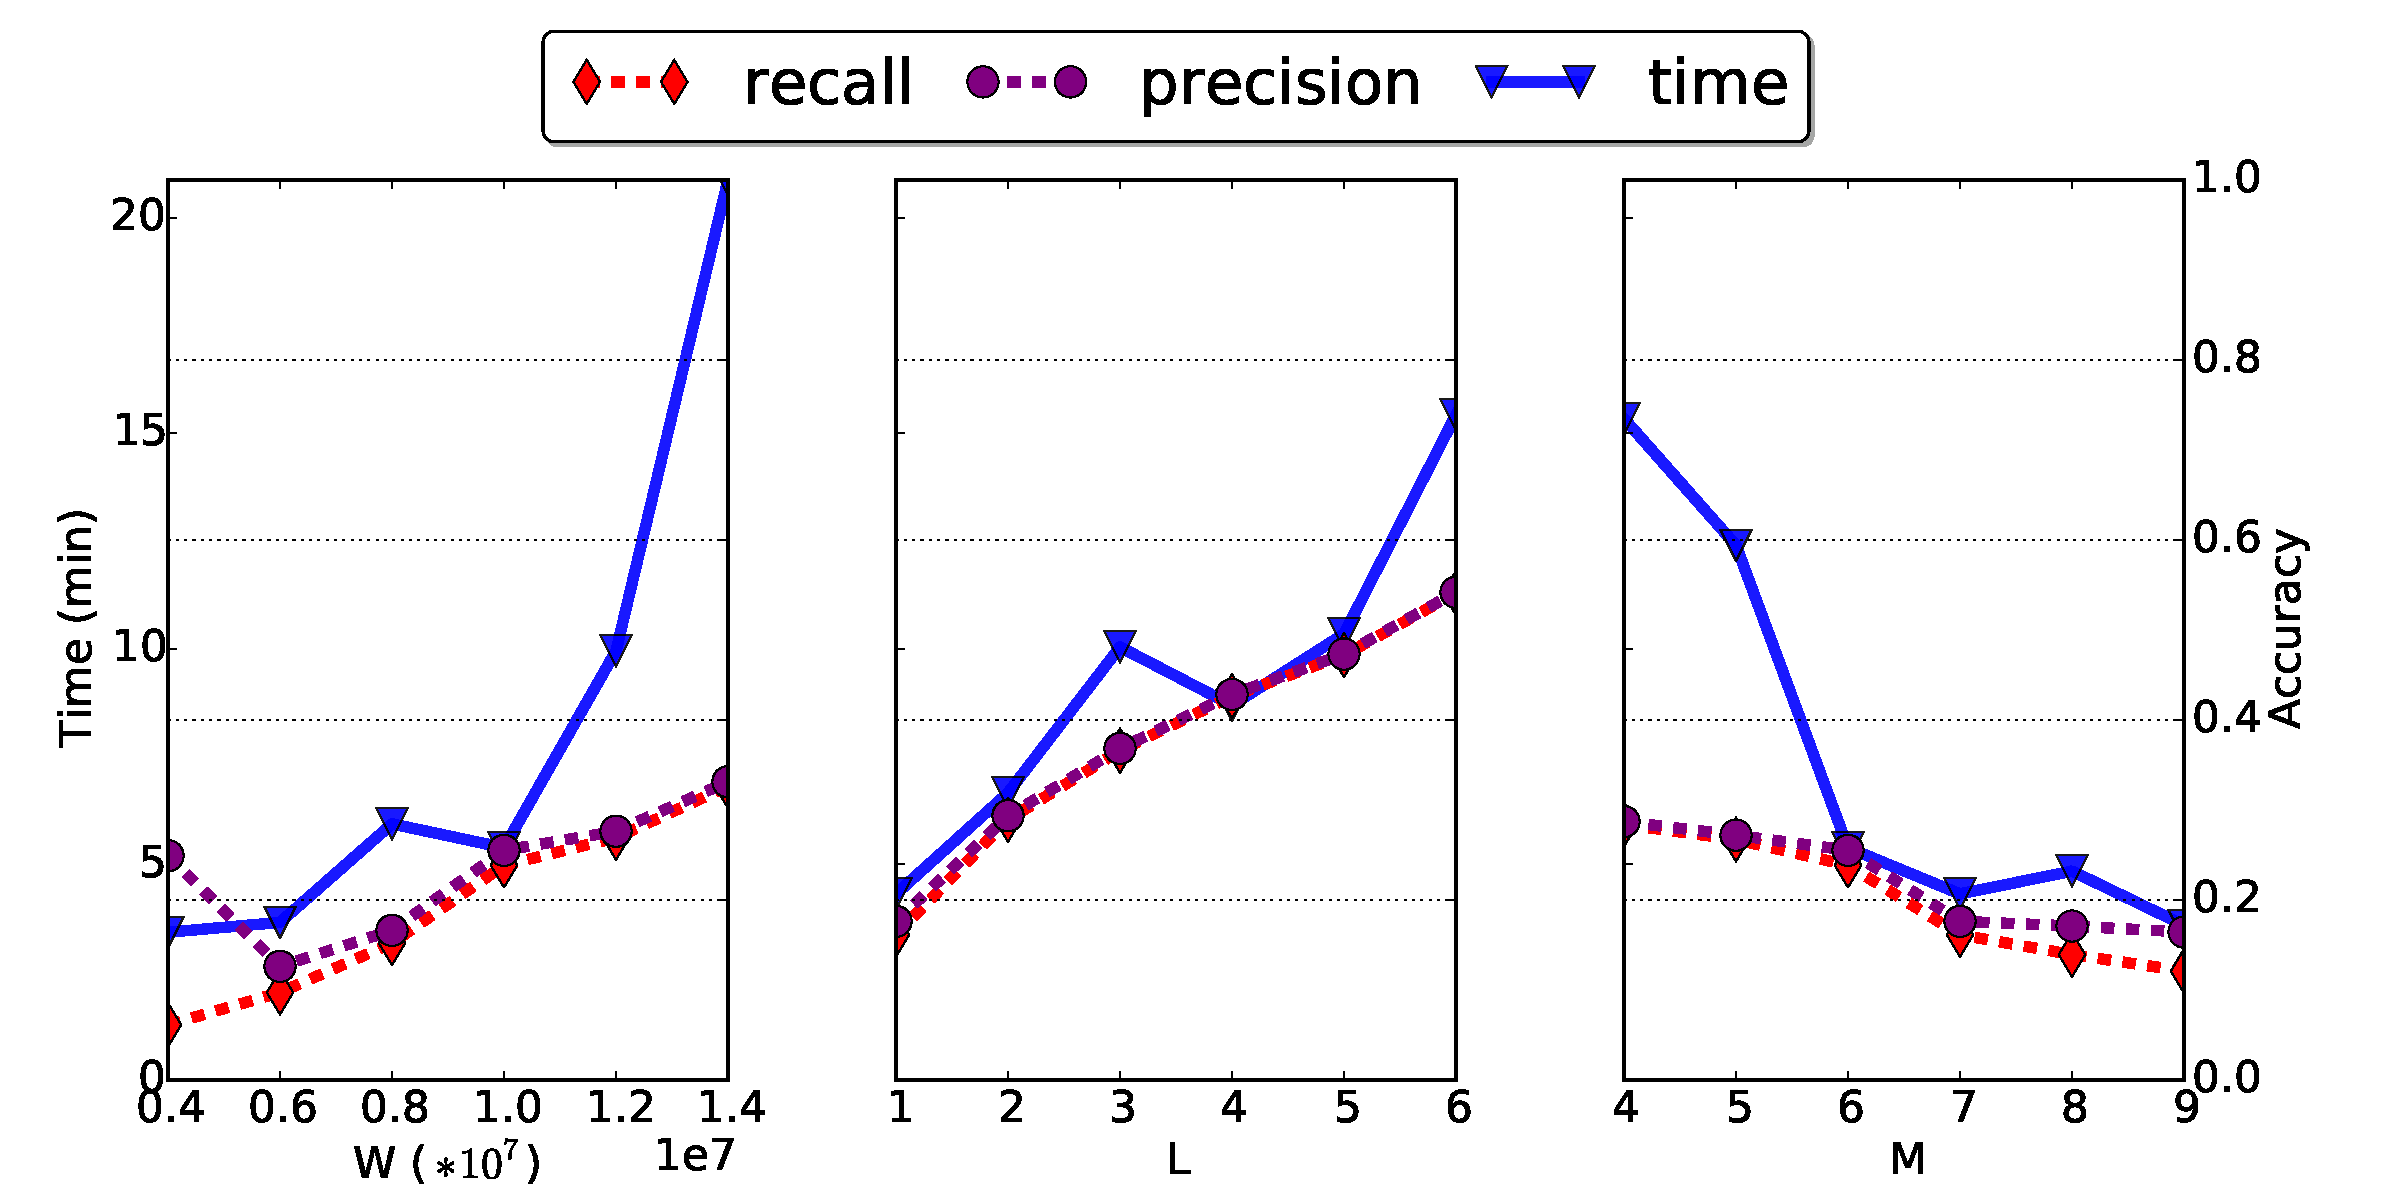
\includegraphics[width=0.5\textwidth]{img-perf/perso/lsh/params_surf.pdf} 
                %\caption{lsh tunning surf}
                \label{dim_acc}
        %\end{subfigure}
         \caption{Impact of parameters on LSH with SURF dataset}
          \label{fig:lsh_tunning_surf}
\end{figure}